\documentclass[11pt,a4paper]{article}
\usepackage[margin=2cm]{geometry}
\usepackage{tikz}
\usetikzlibrary{shapes,arrows.meta,positioning,calc,fit}
\usepackage{tabularx}
\usepackage{longtable}
\usepackage{array}
\usepackage{xcolor}
\usepackage{amsmath,amssymb}
\usepackage{enumitem}
\usepackage{tcolorbox}
\tcbuselibrary{skins,breakable,listings}
\usepackage{listings}
\usepackage{hyperref}
\usepackage{fancyhdr}
\usepackage{titlesec}

\hypersetup{colorlinks=true,linkcolor=blue!50!black,urlcolor=blue!50!black,
  pdftitle={Prolog Lab 6 -- Complete Beginner Guide}}

\setlength{\parindent}{0pt}
\setlength{\parskip}{0.55em}
\renewcommand{\arraystretch}{1.25}
\setcounter{tocdepth}{1}

\pagestyle{fancy}
\fancyhf{}
\fancyhead[L]{\small Prolog Lab 6 -- Beginner's Guide}
\fancyhead[R]{\small \leftmark}
\fancyfoot[C]{\thepage}

\titleformat{\section}{\Large\bfseries\color{blue!50!black}}{\thesection}{0.6em}{}
\titleformat{\subsection}{\large\bfseries\color{black!75}}{\thesubsection}{0.6em}{}

% ---------- inline code ----------
\newcommand{\pred}[1]{\texttt{\detokenize{#1}}}

% ---------- coloured boxes ----------
\newtcolorbox{defbox}[1]{enhanced,breakable,colback=blue!5!white,colframe=blue!60!black,
  fonttitle=\bfseries,title={Definition: #1},left=6pt,right=6pt}
\newtcolorbox{patternbox}[1]{enhanced,breakable,colback=green!6!white,colframe=green!45!black,
  fonttitle=\bfseries,title={Pattern: #1},left=6pt,right=6pt}
\newtcolorbox{mnbox}{enhanced,breakable,colback=orange!8!white,colframe=orange!80!black,
  fonttitle=\bfseries,title={Mnemonic},left=6pt,right=6pt}
\newtcolorbox{warnbox}[1]{enhanced,breakable,colback=red!5!white,colframe=red!60!black,
  fonttitle=\bfseries,title={Watch out: #1},left=6pt,right=6pt}
\newtcolorbox{keybox}{enhanced,breakable,colback=violet!6!white,colframe=violet!60!black,
  fonttitle=\bfseries,title={Key Takeaways},left=6pt,right=6pt}

% ---------- code listings ----------
\lstdefinestyle{pl}{language=Prolog,basicstyle=\ttfamily\small,columns=fullflexible,
  numbers=left,numberstyle=\tiny\color{gray},numbersep=6pt,frame=single,
  backgroundcolor=\color{yellow!8},breaklines=true,showstringspaces=false,
  keywordstyle=\color{blue!70!black},commentstyle=\color{green!40!black}\itshape,
  xleftmargin=1.6em,framexleftmargin=1.6em,aboveskip=0.6em,belowskip=0.4em}
\lstdefinestyle{tr}{language={},basicstyle=\ttfamily\footnotesize,columns=fullflexible,
  frame=single,backgroundcolor=\color{gray!8},breaklines=true,showstringspaces=false,
  aboveskip=0.6em,belowskip=0.4em}
\lstdefinestyle{inl}{language=Prolog,basicstyle=\ttfamily\small,columns=fullflexible,
  frame=single,backgroundcolor=\color{yellow!8},breaklines=true,showstringspaces=false,
  keywordstyle=\color{black},commentstyle=\color{green!40!black}\itshape,
  aboveskip=0.6em,belowskip=0.4em}

% line-by-line helper
\newcommand{\Ln}[1]{\item[Line #1]}
\newenvironment{lines}{\begin{description}[leftmargin=4.5em,style=nextline,font=\bfseries\color{blue!50!black}]}{\end{description}}

% ---------- tikz styles ----------
\tikzset{
  >=Stealth,
  box/.style={draw,rounded corners,fill=blue!8,align=center,minimum width=2.6cm,font=\small,inner sep=4pt},
  dec/.style={draw,diamond,aspect=2.2,fill=yellow!25,align=center,font=\small,inner sep=1pt},
  good/.style={draw,rounded corners,fill=green!15,align=center,font=\small,inner sep=4pt},
  bad/.style={draw,rounded corners,fill=red!12,align=center,font=\small,inner sep=4pt},
  cell/.style={draw,minimum height=0.8cm,minimum width=0.8cm,fill=blue!8},
  person/.style={draw,circle,fill=blue!8,minimum size=0.9cm,font=\small,inner sep=1pt},
  op/.style={draw,rounded corners,fill=orange!15,minimum size=0.8cm,font=\small},
  num/.style={draw,circle,fill=green!12,minimum size=0.8cm,font=\small,inner sep=1pt}
}

\title{\textbf{Prolog Lab 6}\\[0.3em]\Large Fifteen Classic Problems Explained from Scratch\\[0.3em]\large A Complete Beginner's Guide}
\author{}
\date{}

\begin{document}
\maketitle
\thispagestyle{empty}
\vspace{-1.5em}

\begin{tcolorbox}[enhanced,colback=blue!4,colframe=blue!50!black]
\textbf{How to use this guide.}
Part~I teaches every Prolog idea you need, once, in plain language.
Part~II solves the 15 lab problems.
Every problem follows the same eight-part layout:
(1)~Problem Statement, (2)~Prolog Code, (3)~Prolog Concepts Used, (4)~Line-by-Line Explanation,
(5)~How Prolog Works Internally, (6)~Step-by-Step Execution, (7)~Sample Queries and Outputs,
(8)~Key Takeaways.
Each program is also provided as a separate \texttt{.pl} file (\texttt{p01\_factorial.pl} \dots \texttt{p15\_uncle\_aunt.pl}).
\end{tcolorbox}

\tableofcontents
\newpage

% =====================================================================
\part{Prolog Basics You Need for Every Problem}
% =====================================================================

\section{Running Prolog: Programs, Queries and Answers}

\textbf{Prolog} is a \emph{logic programming language}. In languages like C or Python you tell the computer \emph{how} to do something, step by step. In Prolog you describe \emph{what is true} (facts and rules), and then you \emph{ask questions}. Prolog searches for the answer itself.

This guide uses \textbf{SWI-Prolog}, the most popular free implementation.

\begin{enumerate}[leftmargin=*]
  \item Save a program in a text file, for example \texttt{p01\_factorial.pl}.
  \item Start SWI-Prolog in a terminal: \texttt{swipl p01\_factorial.pl} (or start \texttt{swipl} and type \pred{[p01_factorial].} or \pred{consult('p01_factorial.pl').}).
  \item Prolog shows the prompt \pred{?-}. Type a question (a \emph{query}) and end it with a full stop \texttt{.}
\end{enumerate}

\begin{lstlisting}[style=tr]
?- fact(5, F).
F = 120.
\end{lstlisting}

\begin{defbox}{The answers Prolog can give}
\begin{tabularx}{\linewidth}{|l|X|}
\hline
\textbf{Answer} & \textbf{Meaning}\\\hline
\texttt{true.} & The question is true (and there were no variables to report).\\\hline
\texttt{X = value.} & The question is true when the variable \texttt{X} has this value.\\\hline
\texttt{false.} & Prolog searched \emph{every} possibility and found none. This is a normal answer, \emph{not} an error.\\\hline
\texttt{ERROR: \dots} & You made a mistake (for example, an unknown predicate or a variable used in arithmetic before it has a value).\\\hline
\end{tabularx}
\end{defbox}

\begin{warnbox}{the \texttt{;} prompt}
When Prolog gives an answer but still has untried possibilities, it may wait after the answer. Press \textbf{Enter} (or \texttt{.}) to stop, or press \textbf{;} (meaning ``or?'') to ask for another answer. For the deterministic examples in this guide, the extra answer is simply \texttt{false.} In the sample outputs we show the answers only, without these prompts.
\end{warnbox}

\section{The Building Blocks: Terms}

Everything in Prolog is a \textbf{term}. There are only a few kinds:

\begin{center}
\begin{tabularx}{\linewidth}{|l|X|X|}
\hline
\textbf{Kind} & \textbf{Looks like} & \textbf{Notes}\\\hline
Atom & \pred{tom}, \pred{bob}, \pred{add}, \pred{[]} & Starts with a \emph{lowercase} letter. A constant name; it only means itself.\\\hline
Number & \pred{0}, \pred{42}, \pred{-3}, \pred{2.5} & Integers and decimals.\\\hline
Variable & \pred{X}, \pred{Name}, \pred{_}, \pred{_Tmp} & Starts with an \emph{uppercase} letter or underscore. A placeholder that Prolog fills in.\\\hline
Compound term & \pred{parent(tom, bob)}, \pred{add(3, 4)} & A name (the \emph{functor}) followed by arguments in parentheses.\\\hline
List & \pred{[1,2,3]}, \pred{[a,b|T]}, \pred{[]} & An ordered sequence (see Section~\ref{sec:lists}).\\\hline
\end{tabularx}
\end{center}

\begin{mnbox}
\textbf{Capital = Changeable.} If a word starts with a \textbf{C}apital letter it is a variable (it can change). \textbf{l}owercase = \textbf{l}ocked constant.
\end{mnbox}

\section{Facts, Rules, Queries, Predicates}

\begin{defbox}{Fact}
A statement that is unconditionally true. It ends with a full stop.\\
\pred{parent(tom, bob).} reads: ``Tom is a parent of Bob.''
\end{defbox}

\begin{defbox}{Rule}
A statement of the form \pred{Head :- Body.} The symbol \pred{:-} is read ``\emph{if}''. The head is true \emph{if} every goal in the body is true. Goals in the body are separated by commas, and a comma means \textbf{AND}.\\
\pred{grandparent(X, Z) :- parent(X, Y), parent(Y, Z).}\\
reads: ``X is a grandparent of Z if X is a parent of some Y and that Y is a parent of Z.''
\end{defbox}

\begin{defbox}{Query (Goal)}
A question you type at the \pred{?-} prompt, such as \pred{?- parent(tom, bob).} Prolog tries to prove it from your facts and rules.
\end{defbox}

\begin{defbox}{Clause, Predicate, Arity}
A \textbf{clause} is one fact or one rule. A \textbf{predicate} is a group of clauses with the same name and the same number of arguments. The number of arguments is the \textbf{arity}. We write a predicate as \texttt{name/arity}, for example \pred{fact/2}. Note that \pred{eval/2} and \pred{eval/3} would be two different predicates.
\end{defbox}

\textbf{A Prolog program is a database of clauses.} Prolog contains no ``main'' function; you start the computation by asking a query.

\begin{center}
\begin{tabularx}{\linewidth}{|l|X|X|}
\hline
 & \textbf{Fact} & \textbf{Rule}\\\hline
Shape & \pred{head.} & \pred{head :- goal1, goal2.}\\\hline
Meaning & Always true & True only if the body is true\\\hline
Example & \pred{male(tom).} & \pred{uncle(U,C) :- parent(P,C), sibling(U,P), male(U).}\\\hline
\end{tabularx}
\end{center}

\section{Unification: How Prolog Matches Things}

\textbf{Unification} is Prolog's one fundamental operation: ``make these two terms identical, by giving values to variables if necessary.'' It is what the \pred{=} operator does, and it also happens every time Prolog matches a goal against a clause head.

\begin{center}
\begin{tabularx}{\linewidth}{|l|l|X|}
\hline
\textbf{Unify this} & \textbf{With this} & \textbf{Result}\\\hline
\pred{tom} & \pred{tom} & Succeeds (identical atoms)\\\hline
\pred{tom} & \pred{bob} & Fails (different atoms)\\\hline
\pred{X} & \pred{5} & Succeeds, \pred{X = 5}\\\hline
\pred{f(X, 2)} & \pred{f(1, Y)} & Succeeds, \pred{X = 1, Y = 2}\\\hline
\pred{f(X, X)} & \pred{f(1, 2)} & Fails: \pred{X} cannot be both 1 and 2\\\hline
\pred{[H|T]} & \pred{[a,b,c]} & Succeeds, \pred{H = a, T = [b,c]}\\\hline
\pred{[H|T]} & \pred{[]} & Fails (the empty list has no head)\\\hline
\end{tabularx}
\end{center}

Two rules to remember:
\begin{itemize}[leftmargin=*]
  \item A variable can be bound to a value, and once bound it \textbf{keeps} that value (until Prolog backtracks, see below). You cannot ``update'' a variable like \texttt{x = x + 1} in C.
  \item If the same variable appears twice in one clause head, both places must receive the same value. Problem~9 uses this deliberately.
\end{itemize}

\section{How Prolog Executes a Query (The Search Engine)}

Prolog uses a fixed, mechanical procedure. Learn it once and every program becomes predictable.

\begin{defbox}{Prolog's execution rules}
\begin{enumerate}[leftmargin=*]
  \item \textbf{Goals are solved left to right.} In \pred{a, b, c} Prolog solves \pred{a} first, then \pred{b}, then \pred{c}.
  \item \textbf{Clauses are tried top to bottom} in the order they appear in the file.
  \item To solve a goal, Prolog finds a clause whose \emph{head unifies} with the goal. If it is a fact, the goal succeeds. If it is a rule, Prolog now must solve the body goals.
  \item If a goal \textbf{fails}, Prolog \textbf{backtracks}: it goes back to the most recent place where it made a choice (a \emph{choice point}), undoes the variable bindings made since then, and tries the next alternative.
  \item If no alternatives are left anywhere, the original query answers \pred{false}.
\end{enumerate}
\end{defbox}

\begin{center}
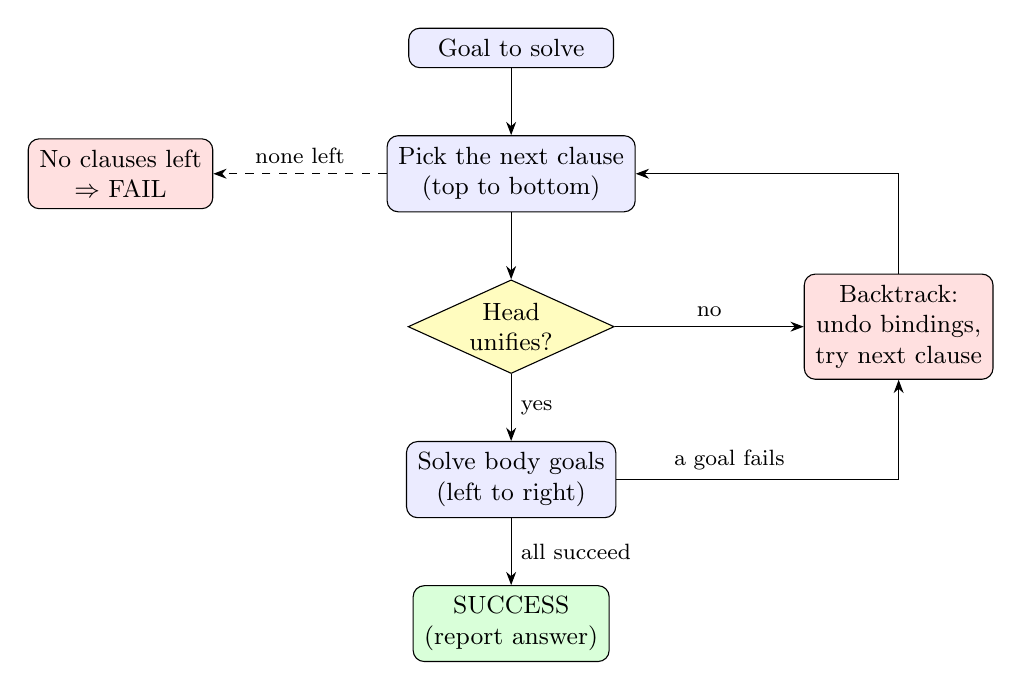
\begin{tikzpicture}[node distance=0.85cm]
\node[box](q){Goal to solve};
\node[box,below=of q](f){Pick the next clause\\(top to bottom)};
\node[dec,below=of f](u){Head\\unifies?};
\node[box,below=of u](b){Solve body goals\\(left to right)};
\node[good,below=of b](s){SUCCESS\\(report answer)};
\node[bad,right=2.4cm of u](bt){Backtrack:\\undo bindings,\\try next clause};
\node[bad,left=2.2cm of f](nf){No clauses left\\$\Rightarrow$ FAIL};
\draw[->](q)--(f);
\draw[->](f)--(u);
\draw[->](u)--(b) node[midway,right,font=\footnotesize]{yes};
\draw[->](b)--(s) node[midway,right,font=\footnotesize]{all succeed};
\draw[->](u)--(bt) node[midway,above,font=\footnotesize]{no};
\draw[->](b.east) -| (bt.south) node[pos=0.2,above,font=\footnotesize]{a goal fails};
\draw[->](bt.north) |- (f.east);
\draw[->,dashed](f.west)--(nf.east) node[midway,above,font=\footnotesize]{none left};
\end{tikzpicture}
\end{center}

\textbf{Choice points.} When more than one clause could match, Prolog remembers the untried clauses. If the current attempt later fails, or if you press \texttt{;}, Prolog resumes from that memory. This automatic try-and-retry is called \textbf{backtracking}.

\textbf{Fresh variables.} Each time Prolog uses a clause it makes a \emph{private copy} of the clause with brand-new variables. This is why a recursive rule can call itself: the \pred{N} in one call is a different variable from the \pred{N} in the next call.

\section{Recursion}

A \textbf{recursive} predicate calls itself on a smaller problem. Because Prolog has no loops (\texttt{for}, \texttt{while}), recursion is how you repeat work. Every correct recursive predicate has two parts:

\begin{patternbox}{Base case + recursive case}
\begin{enumerate}[leftmargin=*]
  \item \textbf{Base case}: the smallest problem, answered directly (usually a fact). It stops the recursion.
  \item \textbf{Recursive case}: reduces the problem to a smaller one, calls itself, then combines the result.
\end{enumerate}
\end{patternbox}

\textbf{The call stack.} Prolog remembers each unfinished call, like a stack of plates. Calls pile up until the base case is reached; then answers are passed back down, one call at a time. In the factorial problem you will see this drawn.

\begin{mnbox}
\textbf{B-R-C:} \textbf{B}ase case first, \textbf{R}ecurse on something smaller, \textbf{C}ombine the result. If you forget the smaller step, the program runs forever (stack overflow).
\end{mnbox}

\section{Lists}\label{sec:lists}

A list is written in square brackets: \pred{[a,b,c]}. The empty list is \pred{[]}. Internally, a list is a chain: a \textbf{Head} (first element) joined to a \textbf{Tail} (the rest of the list, which is itself a list). The notation \pred{[H|T]} splits a list into these two parts; the vertical bar \pred{|} is read ``followed by''.

\begin{center}
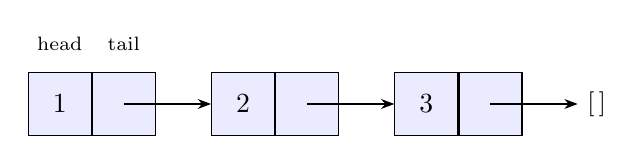
\begin{tikzpicture}[node distance=0pt]
\node[cell](h1){1};\node[cell,right=of h1](t1){};
\node[cell,right=0.7cm of t1](h2){2};\node[cell,right=of h2](t2){};
\node[cell,right=0.7cm of t2](h3){3};\node[cell,right=of h3](t3){};
\node[right=0.7cm of t3,font=\small](nil){[\,]};
\draw[->](t1.center)--(h2.west);
\draw[->](t2.center)--(h3.west);
\draw[->](t3.center)--(nil.west);
\node[above=0.15cm of h1,font=\scriptsize]{head};
\node[above=0.15cm of t1,font=\scriptsize]{tail};
\end{tikzpicture}
\end{center}

\begin{center}
\begin{tabularx}{\linewidth}{|l|X|X|}
\hline
\textbf{Pattern} & \textbf{Matches} & \textbf{Example match with \pred{[a,b,c]}}\\\hline
\pred{[]} & only the empty list & no match\\\hline
\pred{[X]} & a list of exactly one element & no match (3 elements)\\\hline
\pred{[H|T]} & any non-empty list & \pred{H = a, T = [b,c]}\\\hline
\pred{[X,Y|T]} & a list with at least two elements & \pred{X = a, Y = b, T = [c]}\\\hline
\pred{[_|T]} & non-empty list, ignore the head & \pred{T = [b,c]}\\\hline
\end{tabularx}
\end{center}

\begin{patternbox}{The standard list recursion}
\begin{lstlisting}[style=inl]
process([], BaseAnswer).                  % empty list
process([H|T], Answer) :-
    process(T, AnswerForTail),            % solve the smaller list
    combine(H, AnswerForTail, Answer).    % use the head + tail answer
\end{lstlisting}
Almost every list problem in this guide (Problems 2--6, 9, 11, 12) is a variation of this shape.
\end{patternbox}

\section{Arithmetic and Comparison}

\begin{warnbox}{\texttt{=} does not calculate}
In Prolog, \pred{X = 2 + 3} does \emph{not} give 5. It just unifies \pred{X} with the term \pred{2+3}. To calculate, use \pred{is}.
\end{warnbox}

\begin{center}
\begin{tabularx}{\linewidth}{|l|X|X|}
\hline
\textbf{Operator} & \textbf{What it does} & \textbf{Example}\\\hline
\pred{=} & Unifies two terms (no calculation) & \pred{X = 2+3} gives \pred{X = 2+3}\\\hline
\pred{\=} & Succeeds if two terms \emph{cannot} unify & \pred{a \= b} is true\\\hline
\pred{is} & Calculates the right side, unifies result with the left & \pred{X is 2+3} gives \pred{X = 5}\\\hline
\pred{=:=} & Arithmetic equal & \pred{4 =:= 2+2} is true\\\hline
\pred{=\=} & Arithmetic not equal & \pred{3 =\= 2+2} is true\\\hline
\pred{<  >  =<  >=} & Arithmetic comparison & \pred{3 =< 3} is true\\\hline
\end{tabularx}
\end{center}

Useful arithmetic functions: \pred{+ - * /}, \pred{mod} (remainder, so \pred{7 mod 2 =:= 1}), and \pred{max(A,B)}.

\textbf{Important rules.}
\begin{itemize}[leftmargin=*]
  \item The right side of \pred{is} (and both sides of \pred{<}, \pred{=:=}, etc.) must contain only numbers or variables that \emph{already have numeric values}. Otherwise Prolog reports an error.
  \item ``Less than or equal'' is written \pred{=<}, \emph{not} \pred{<=}.
  \item The left side of \pred{is} is normally a fresh variable: write \pred{N1 is N - 1}, never \pred{N is N - 1} (that would try to give \pred{N} a second value).
\end{itemize}

\begin{mnbox}
\textbf{``= matches, is calculates, =:= compares.''} Also: the arrow of \textbf{less-or-equal points to the equal sign}: \pred{=<}.
\end{mnbox}

\section{Negation and the Anonymous Variable}

\textbf{Negation as failure:} \pred{\+ Goal} succeeds when Prolog \emph{cannot prove} \pred{Goal}. Read \pred{\+} as ``it is not provable that''. Problem~13 uses it.

\textbf{Anonymous variable:} a single underscore \pred{_} means ``some value, but I do not care what.'' Every \pred{_} is independent of every other \pred{_}. Using it avoids ``singleton variable'' warnings for variables that appear only once.

\section{Collecting All Answers: \texttt{findall/3} and \texttt{sort/2}}

Normally Prolog gives answers one at a time. The predicate \pred{findall(Template, Goal, List)} runs \pred{Goal} and \emph{collects every solution} into \pred{List}. Here, \pred{Template} says which variable's value you want to save from each solution.

\begin{lstlisting}[style=tr]
?- findall(X, member(X, [a,b,c]), L).
L = [a, b, c].
\end{lstlisting}

If there are no solutions, \pred{findall} succeeds with the empty list \pred{[]}.

\pred{sort(List, Sorted)} puts the list in standard order \emph{and removes duplicates}. Problem~10 relies on this.

\section{Quick Reference Tables}

\begin{center}
\begin{tabularx}{\linewidth}{|l|X|X|}
\hline
\textbf{Problem you hit} & \textbf{Typical cause} & \textbf{Fix}\\\hline
\pred{Unknown procedure foo/2} & Misspelled name or wrong arity & Check spelling and argument count\\\hline
\pred{Arguments are not sufficiently instantiated} & A variable used in \pred{is} or \pred{<} has no value yet & Make sure the variable is bound earlier in the body\\\hline
Program never stops / stack overflow & Missing base case, or the recursive step does not shrink the problem & Add a base case; shrink the argument\\\hline
Unexpected \pred{false} & Order of goals wrong, or a guard such as \pred{N > 0} fails & Test sub-goals one at a time\\\hline
Singleton variable warning & A variable appears only once in a clause & Rename it to \pred{_} or fix a typo\\\hline
\end{tabularx}
\end{center}

\textbf{Want to watch Prolog think?} Type \pred{trace.} then your query. Prolog prints every \texttt{Call}, \texttt{Exit}, \texttt{Redo} and \texttt{Fail} step. Type \pred{notrace.} to stop. The step-by-step sections in Part~II mimic what this trace shows.

\begin{mnbox}
\textbf{Prolog's four port words: C-E-R-F} (``\textbf{C}all, \textbf{E}xit, \textbf{R}edo, \textbf{F}ail''): Call starts a goal, Exit means it succeeded, Redo means ``try another way'', Fail means no way worked.
\end{mnbox}

\newpage

\part{The Fifteen Problems}
\setcounter{section}{0}
\renewcommand{\thesection}{\arabic{section}}
\renewcommand{\thesubsection}{\arabic{subsection}}
\titleformat{\section}{\Large\bfseries\color{blue!50!black}}{Problem \thesection:}{0.5em}{}
\titleformat{\subsection}{\large\bfseries\color{black!75}}{\thesubsection.}{0.5em}{}

% =====================================================================
\section{Factorial Calculation (Recursion)}
% =====================================================================
\setcounter{subsection}{0}
\subsection{Problem Statement}
Write a Prolog program to calculate the factorial of a number using recursion.

\begin{defbox}{Factorial}
$n! = n \times (n-1) \times \dots \times 2 \times 1$, and by definition $0! = 1$.\\
Example: $5! = 5\times4\times3\times2\times1 = 120$. Notice that $n! = n \times (n-1)!$. This self-reference is exactly what recursion needs.
\end{defbox}

\subsection{Prolog Code}
File: \texttt{p01\_factorial.pl}
\begin{lstlisting}[style=pl]
fact(0, 1).                  % base case: 0! = 1
fact(N, F) :-                % recursive case
    N > 0,
    N1 is N - 1,
    fact(N1, F1),
    F is N * F1.
\end{lstlisting}

\subsection{Prolog Concepts Used}
\begin{itemize}[leftmargin=*]
  \item \textbf{Fact} (line 1) and \textbf{rule} (lines 2--6).
  \item \textbf{Recursion} with a base case and a recursive case.
  \item \textbf{Arithmetic with \pred{is}} and the comparison \pred{>}.
  \item \textbf{Guard}: a test (\pred{N > 0}) that decides whether a clause is allowed to apply.
  \item \textbf{Fresh variables per call}: each recursive call has its own \pred{N}, \pred{N1}, \pred{F}, \pred{F1}.
\end{itemize}

\subsection{Line-by-Line Explanation}
\begin{lines}
\Ln{1} \pred{fact(0, 1).} A fact: ``the factorial of 0 is 1.'' This is the \textbf{base case}; the recursion stops here.
\Ln{2} \pred{fact(N, F) :-} The head of the \textbf{recursive rule}: ``the factorial of \pred{N} is \pred{F}, \emph{if} the goals below are all true.'' \pred{N} is the input, \pred{F} the output.
\Ln{3} \pred{N > 0,} A guard. It makes sure we only recurse for positive numbers. (Without it, a negative input would recurse forever.)
\Ln{4} \pred{N1 is N - 1,} Calculates $N-1$ and stores it in the new variable \pred{N1}. This is the \emph{smaller problem}.
\Ln{5} \pred{fact(N1, F1),} The recursive call: ``let \pred{F1} be the factorial of \pred{N1}.''
\Ln{6} \pred{F is N * F1.} Once \pred{F1} is known, compute $N \times F1$ and give it to \pred{F}. This uses the identity $n! = n \times (n-1)!$.
\end{lines}

\subsection{How Prolog Works Internally}
\begin{enumerate}[leftmargin=*]
  \item \textbf{Matching the goal to clauses.} For the goal \pred{fact(3, F)}, Prolog tries clause 1 first: can \pred{fact(0, 1)} unify with \pred{fact(3, F)}? No, because $3 \neq 0$. So Prolog moves on to clause 2, whose head \pred{fact(N, F)} unifies with anything, giving \pred{N = 3}.
  \item \textbf{Solving the body left to right.} \pred{3 > 0} is true. \pred{N1 is 3-1} binds \pred{N1 = 2}. Then comes the recursive goal \pred{fact(2, F1)}. Prolog must finish it before it can look at the last line.
  \item \textbf{Fresh variables.} The new call uses a renamed copy of the clause, so you can picture \pred{N_2, F_2, N1_2, F1_2}. The values from the first call are not disturbed.
  \item \textbf{The stack builds up.} The calls for $3, 2, 1, 0$ wait for each other. Only \pred{fact(0, F)} can be answered immediately (clause 1).
  \item \textbf{The answer is built on the way back.} Each waiting call now finishes its last line \pred{F is N * F1} and hands its result to the caller.
  \item \textbf{Why the guard matters.} The goal \pred{fact(-1, F)} matches clause 2, but \pred{-1 > 0} fails, so Prolog answers \pred{false}. Without the guard, the sequence $-1, -2, -3, \dots$ would never reach 0 and Prolog would run out of memory.
\end{enumerate}

\begin{center}
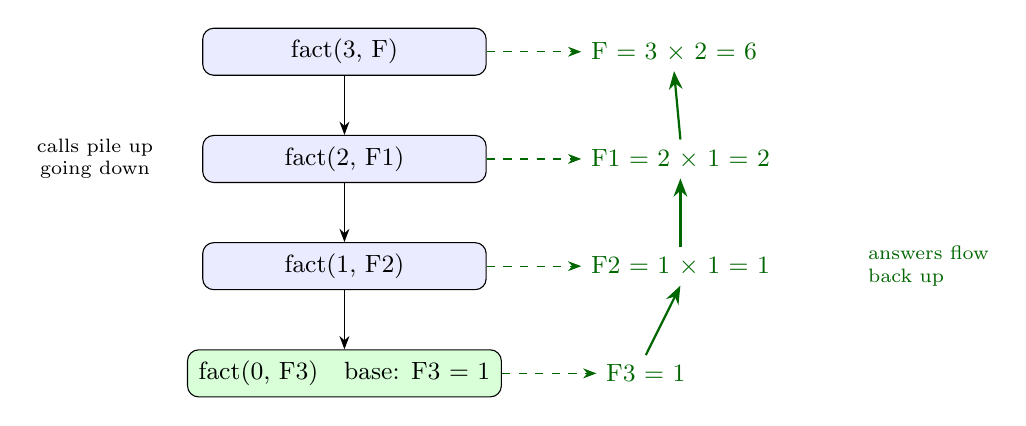
\begin{tikzpicture}[node distance=0.75cm]
\node[box,minimum width=3.6cm](a){fact(3, F)};
\node[box,minimum width=3.6cm,below=of a](b){fact(2, F1)};
\node[box,minimum width=3.6cm,below=of b](c){fact(1, F2)};
\node[good,minimum width=3.6cm,below=of c](d){fact(0, F3)\quad base: F3 = 1};
\draw[->](a)--(b);\draw[->](b)--(c);\draw[->](c)--(d);
\node[left=0.5cm of b,font=\scriptsize,align=center]{calls pile up\\going down};
\node[right=1.2cm of d,font=\small,text=green!40!black](r3){F3 = 1};
\node[right=1.2cm of c,font=\small,text=green!40!black](r2){F2 = 1 $\times$ 1 = 1};
\node[right=1.2cm of b,font=\small,text=green!40!black](r1){F1 = 2 $\times$ 1 = 2};
\node[right=1.2cm of a,font=\small,text=green!40!black](r0){F = 3 $\times$ 2 = 6};
\draw[->,dashed,green!40!black](d.east)--(r3.west);
\draw[->,dashed,green!40!black](c.east)--(r2.west);
\draw[->,dashed,green!40!black](b.east)--(r1.west);
\draw[->,dashed,green!40!black](a.east)--(r0.west);
\draw[->,green!40!black,thick](r3.north)--(r2.south);
\draw[->,green!40!black,thick](r2.north)--(r1.south);
\draw[->,green!40!black,thick](r1.north)--(r0.south);
\node[right=0.1cm of r2,font=\scriptsize,green!40!black,align=left,xshift=0.9cm]{answers flow\\back up};
\end{tikzpicture}
\end{center}

\subsection{Step-by-Step Execution / Query Flow}
Query: \pred{?- fact(3, F).}

\begin{lstlisting}[style=tr]
CALL fact(3, F)
  clause 1 fact(0,1)?  3 vs 0 -> no match
  clause 2 fact(N,F):  N = 3
    3 > 0                  -> true
    N1 is 3 - 1            -> N1 = 2
    CALL fact(2, F1)
      clause 1?  2 vs 0 -> no.   clause 2: N = 2
        2 > 0                -> true
        N1 is 2 - 1          -> N1 = 1
        CALL fact(1, F2)
          clause 1?  1 vs 0 -> no.   clause 2: N = 1
            1 > 0              -> true
            N1 is 1 - 1        -> N1 = 0
            CALL fact(0, F3)
              clause 1 fact(0,1) matches -> F3 = 1   (EXIT)
            F2 is 1 * 1        -> F2 = 1               (EXIT)
        F1 is 2 * 1          -> F1 = 2                 (EXIT)
    F is 3 * 2             -> F = 6                    (EXIT)
Answer: F = 6.
\end{lstlisting}

\textbf{Worked numerical problem.} Compute \pred{fact(5, F)} by hand: the calls go $5 \to 4 \to 3 \to 2 \to 1 \to 0$. The base case gives 1. Coming back: $1\times1=1$, $2\times1=2$, $3\times2=6$, $4\times6=24$, $5\times24=\mathbf{120}$.

\subsection{Sample Queries and Outputs}
\begin{lstlisting}[style=tr]
?- fact(5, F).
F = 120.

?- fact(0, F).
F = 1.

?- fact(10, F).
F = 3628800.

?- fact(-3, F).
false.

?- fact(4, 24).       % checking an answer instead of computing one
true.
\end{lstlisting}

\begin{keybox}
\begin{itemize}[leftmargin=*]
  \item Base case first (\pred{fact(0,1)}), then the recursive rule.
  \item The recursive call must work on a \emph{smaller} number (\pred{N1 is N-1}).
  \item The result is combined \emph{after} the recursive call returns.
  \item The guard \pred{N > 0} protects against endless recursion.
\end{itemize}
\end{keybox}
\begin{mnbox}
\textbf{``Zero is one, then times down.''} $0! = 1$, and each level multiplies by the answer from below.
\end{mnbox}

\newpage
% =====================================================================
\section{Sum of Even Numbers in a List}
% =====================================================================
\setcounter{subsection}{0}
\subsection{Problem Statement}
Define a predicate \pred{sum_even(List, Sum)} that returns the sum of all even numbers in a given list.

\subsection{Prolog Code}
File: \texttt{p02\_sum\_even.pl}
\begin{lstlisting}[style=pl]
sum_even([], 0).                    % empty list: sum is 0
sum_even([H|T], Sum) :-             % H is even: add it
    H mod 2 =:= 0,
    sum_even(T, Rest),
    Sum is Rest + H.
sum_even([H|T], Sum) :-             % H is odd: skip it
    H mod 2 =\= 0,
    sum_even(T, Sum).
\end{lstlisting}

\subsection{Prolog Concepts Used}
\begin{itemize}[leftmargin=*]
  \item \textbf{List recursion} with \pred{[]} as the base case and \pred{[H|T]} to take the list apart.
  \item \textbf{\pred{mod}} (remainder after division): a number is even when \pred{H mod 2 =:= 0}.
  \item \textbf{Arithmetic comparison} \pred{=:=} (equal) and \pred{=\=} (not equal).
  \item \textbf{Two rules for one pattern}, separated by mutually exclusive guards (even versus odd).
\end{itemize}

\subsection{Line-by-Line Explanation}
\begin{lines}
\Ln{1} \pred{sum_even([], 0).} The sum of an empty list is 0. Base case.
\Ln{2} \pred{sum_even([H|T], Sum) :-} Rule for a non-empty list. \pred{H} is the first element, \pred{T} the rest. This clause handles the case where the first element is even.
\Ln{3} \pred{H mod 2 =:= 0,} Guard: the remainder of \pred{H} divided by 2 is 0, so \pred{H} is even.
\Ln{4} \pred{sum_even(T, Rest),} Recursively compute the sum of evens in the tail and call it \pred{Rest}.
\Ln{5} \pred{Sum is Rest + H.} Since \pred{H} is even, add it to the tail's sum.
\Ln{6} \pred{sum_even([H|T], Sum) :-} Second rule for a non-empty list: the case where the first element is not even.
\Ln{7} \pred{H mod 2 =\= 0,} Guard: the remainder is not 0, so \pred{H} is odd.
\Ln{8} \pred{sum_even(T, Sum).} Skip \pred{H}. The sum of the whole list equals the sum of the tail, so the \emph{same} variable \pred{Sum} is passed along unchanged.
\end{lines}

\subsection{How Prolog Works Internally}
\begin{itemize}[leftmargin=*]
  \item For a non-empty list, \emph{both} clause 2 and clause 3 have heads that unify. Prolog tries clause 2 first (top to bottom) and leaves a \textbf{choice point} for clause 3.
  \item If \pred{H} is odd, the guard on line 3 fails. Prolog \textbf{backtracks} to the choice point and tries clause 3, whose guard succeeds.
  \item If \pred{H} is even, clause 2 succeeds. Clause 3 stays on the shelf; if it were ever tried, its guard \pred{H mod 2 =\= 0} would fail, so no wrong second answer can appear.
  \item The recursion shrinks the list by one element each time and finally reaches \pred{[]}, matched by line 1.
\end{itemize}

\begin{warnbox}{why both clauses need a guard}
Suppose line 7 were missing. For the query \pred{sum_even([2], S)}, Prolog would give \pred{S = 2}; then, on pressing \texttt{;}, clause 3 would also match and give \pred{S = 0}, which is a wrong second answer. The guard makes the two cases \emph{mutually exclusive}.
\end{warnbox}

\subsection{Step-by-Step Execution / Query Flow}
Query: \pred{?- sum_even([1,2,3,4], S).}

\begin{lstlisting}[style=tr]
sum_even([1,2,3,4], S)
  clause 1: [] vs [1,2,3,4]   -> no
  clause 2: H=1, T=[2,3,4];  1 mod 2 =:= 0 ?   1 =:= 0 -> fails
  clause 3: H=1;             1 mod 2 =\= 0 ?   true
    sum_even([2,3,4], S)
      clause 2: H=2;  2 mod 2 =:= 0 -> true
        sum_even([3,4], Rest)
          clause 2: H=3; 1 =:= 0 -> fails
          clause 3: H=3; odd -> true
            sum_even([4], Rest)
              clause 2: H=4; 0 =:= 0 -> true
                sum_even([], Rest4) -> clause 1: Rest4 = 0
                Sum is 0 + 4 -> Rest = 4
      Sum is 4 + 2 -> S = 6
Answer: S = 6.
\end{lstlisting}

\textbf{Worked numerical problem.} For \pred{[1,2,3,4,5,6]}: the evens are $2, 4, 6$, so the sum is $2+4+6 = \mathbf{12}$. Prolog computes it as $0 + 6 = 6$, then $6+4=10$, then $10+2=12$ (odd elements pass the value unchanged).

\subsection{Sample Queries and Outputs}
\begin{lstlisting}[style=tr]
?- sum_even([1,2,3,4,5,6], S).
S = 12.

?- sum_even([1,3,5], S).
S = 0.

?- sum_even([], S).
S = 0.

?- sum_even([10,-4,7], S).
S = 6.
\end{lstlisting}

\begin{keybox}
\begin{itemize}[leftmargin=*]
  \item Typical list recursion: empty list is the base case; otherwise take \pred{[H|T]}.
  \item Use \emph{two} rules when the head needs a different treatment, and make their guards opposite.
  \item Skipping an element means passing the \emph{same} result variable to the recursive call.
\end{itemize}
\end{keybox}
\begin{mnbox}
\textbf{``Even: add it. Odd: let it go.''}
\end{mnbox}

\newpage
% =====================================================================
\section{Palindrome Checker}
% =====================================================================
\setcounter{subsection}{0}
\subsection{Problem Statement}
Write a predicate \pred{palindrome(List)} that succeeds if the given list is a palindrome (reads the same forwards and backwards, for example \pred{[r,a,c,e,c,a,r]}).

\subsection{Prolog Code}
File: \texttt{p03\_palindrome.pl}
\begin{lstlisting}[style=pl]
palindrome(List) :-
    reverse_list(List, List).        % a palindrome equals its own reverse

reverse_list(List, Reversed) :-
    reverse_acc(List, [], Reversed).
reverse_acc([], Acc, Acc).
reverse_acc([H|T], Acc, Reversed) :-
    reverse_acc(T, [H|Acc], Reversed).
\end{lstlisting}

\subsection{Prolog Concepts Used}
\begin{itemize}[leftmargin=*]
  \item \textbf{Simplest idea:} a list is a palindrome exactly when it \emph{equals its own reverse}.
  \item \textbf{Unification as an equality test}: using the same variable twice forces both places to match.
  \item \textbf{Helper predicates} and \textbf{accumulators} (to reverse a list).
  \item \textbf{Reusing} one predicate inside another.
\end{itemize}

\subsection{Line-by-Line Explanation}
\begin{lines}
\Ln{1} \pred{palindrome(List) :-} ``\pred{List} is a palindrome if the goal below holds.''
\Ln{2} \pred{reverse_list(List, List).} Reverse \pred{List} and demand that the reversed result be \pred{List} again. Writing the \emph{same variable} in both argument positions is the equality test.
\Ln{3} A blank line (ignored by Prolog; it only separates the helper predicates).
\Ln{4} \pred{reverse_list(List, Reversed) :-} A user-friendly wrapper: reverse \pred{List} to give \pred{Reversed}.
\Ln{5} \pred{reverse_acc(List, [], Reversed).} Starts the real work with an \emph{accumulator} (a collecting list) that begins as the empty list \pred{[]}.
\Ln{6} \pred{reverse_acc([], Acc, Acc).} When the input is used up, the accumulator \emph{is} the reversed list, so the two last arguments must be equal.
\Ln{7} \pred{reverse_acc([H|T], Acc, Reversed) :-} Otherwise take the head \pred{H}\ldots
\Ln{8} \pred{reverse_acc(T, [H|Acc], Reversed).} \ldots put \pred{H} on the \emph{front} of the accumulator, and continue with the tail. Because each new head is placed in front, the order flips.
\end{lines}

\subsection{How Prolog Works Internally}
\begin{itemize}[leftmargin=*]
  \item In \pred{palindrome([a,b,a])}, the call on line 2 becomes \pred{reverse_list([a,b,a],[a,b,a])}. So the \emph{third} argument of \pred{reverse_acc} is already known: \pred{[a,b,a]}.
  \item Prolog builds the reversed list in the accumulator (second argument) while walking down the input. It does not use the known third argument until the base case.
  \item At the base case (line 6), the head \pred{reverse_acc([], Acc, Acc)} forces the accumulator and the third argument to \textbf{unify}. If they are the same list, unification succeeds; if not, it fails, and Prolog answers \pred{false}.
  \item After a failure Prolog backtracks, but no other clause can match (line 7 needs a non-empty list), so the final answer is \pred{false}.
\end{itemize}

\subsection{Step-by-Step Execution / Query Flow}
Query: \pred{?- palindrome([a,b,a]).}

\begin{lstlisting}[style=tr]
palindrome([a,b,a])
 -> reverse_list([a,b,a], [a,b,a])
 -> reverse_acc([a,b,a], [],    [a,b,a])    H=a  T=[b,a]
 -> reverse_acc([b,a],   [a],   [a,b,a])    H=b  T=[a]
 -> reverse_acc([a],     [b,a], [a,b,a])    H=a  T=[]
 -> reverse_acc([],      [a,b,a],[a,b,a])   base clause: Acc=[a,b,a]
                                            third arg [a,b,a] -> unify OK
Answer: true.
\end{lstlisting}

Now a failing example, \pred{?- palindrome([a,b,c]).}
\begin{lstlisting}[style=tr]
reverse_acc([a,b,c], [],      [a,b,c])
reverse_acc([b,c],   [a],     [a,b,c])
reverse_acc([c],     [b,a],   [a,b,c])
reverse_acc([],      [c,b,a], [a,b,c])   base clause: Acc=[c,b,a]
                                         third arg [a,b,c] -> [c,b,a] vs [a,b,c]
                                         unification FAILS -> no other clause
Answer: false.
\end{lstlisting}

\subsection{Sample Queries and Outputs}
\begin{lstlisting}[style=tr]
?- palindrome([r,a,c,e,c,a,r]).
true.

?- palindrome([1,2,3]).
false.

?- palindrome([]).
true.

?- palindrome([x]).
true.
\end{lstlisting}

\begin{keybox}
\begin{itemize}[leftmargin=*]
  \item Break a problem into an idea you already know: palindrome = ``equals its reverse''.
  \item The same variable in two argument positions makes Prolog test equality by unification.
  \item The accumulator trick (collect while walking down) reverses a list efficiently.
\end{itemize}
\end{keybox}
\begin{mnbox}
\textbf{``Reverse it and compare''} (Rotor, level, and 12321 are palindromes).
\end{mnbox}

\newpage
% =====================================================================
\section{Maximum Element in a List}
% =====================================================================
\setcounter{subsection}{0}
\subsection{Problem Statement}
Write a predicate \pred{max_list(List, Max)} to find the largest number in a list using recursion.

\subsection{Prolog Code}
File: \texttt{p04\_max\_list.pl}
\begin{lstlisting}[style=pl]
max_list([X], X).                    % one element: it is the maximum
max_list([H|T], Max) :-
    max_list(T, MaxTail),            % maximum of the rest
    Max is max(H, MaxTail).          % bigger of H and that maximum
\end{lstlisting}

\subsection{Prolog Concepts Used}
\begin{itemize}[leftmargin=*]
  \item \textbf{List recursion} where the base case is a \emph{one-element} list, not an empty one.
  \item \textbf{Pattern \pred{[X]}} (a list with exactly one element).
  \item The built-in arithmetic function \pred{max(A, B)} used with \pred{is}.
  \item \textbf{Solving the tail first}, then combining with the head.
\end{itemize}

\textbf{Note.} SWI-Prolog also has a library predicate with the same name. A definition written in your own file takes priority, so the program above works as expected.

\subsection{Line-by-Line Explanation}
\begin{lines}
\Ln{1} \pred{max_list([X], X).} A list with just one element: that element is the maximum. Notice how the same variable \pred{X} appears twice.
\Ln{2} \pred{max_list([H|T], Max) :-} Rule for longer lists: \pred{H} is the first element, \pred{T} the rest.
\Ln{3} \pred{max_list(T, MaxTail),} Find the maximum of the rest of the list.
\Ln{4} \pred{Max is max(H, MaxTail).} The overall maximum is the larger of the head and the tail's maximum.
\end{lines}

\subsection{How Prolog Works Internally}
\begin{itemize}[leftmargin=*]
  \item The empty list \pred{[]} has no maximum, so there is deliberately no clause for it. The goal \pred{max_list([], M)} simply fails.
  \item For \pred{max_list([5], M)}, line 1 matches: \pred{[X]} unifies with \pred{[5]} giving \pred{X = 5}, then the second argument \pred{X} unifies with \pred{M}, giving \pred{M = 5}.
  \item For a list with two or more elements, line 1 cannot match (the list is not of the form \pred{[X]}), so Prolog uses line 2 and recurses on the tail.
  \item For a one-element tail, line 2 \emph{also} matches \pred{[H|T]} with \pred{T = []}. This leaves a harmless choice point: if tried, \pred{max_list([], _)} immediately fails.
  \item The answer is built \emph{while returning}: each level compares its own head with the answer from below.
\end{itemize}

\subsection{Step-by-Step Execution / Query Flow}
Query: \pred{?- max_list([3,9,2], M).}
\begin{lstlisting}[style=tr]
max_list([3,9,2], M)
  clause 1 [X] vs [3,9,2]: tail is not [] -> no match
  clause 2: H=3, T=[9,2]
    max_list([9,2], MaxTail)
      clause 2: H=9, T=[2]
        max_list([2], MaxTail2)
          clause 1: X=2 -> MaxTail2 = 2
        Max is max(9, 2) -> 9
    Max is max(3, 9) -> 9
Answer: M = 9.
\end{lstlisting}

\textbf{Worked numerical problem.} \pred{max_list([4,1,7,3], M)}: tail results come back as $3$; then $\max(7,3)=7$; then $\max(1,7)=7$; then $\max(4,7)=\mathbf{7}$.

\subsection{Sample Queries and Outputs}
\begin{lstlisting}[style=tr]
?- max_list([3,9,2,7], M).
M = 9.

?- max_list([5], M).
M = 5.

?- max_list([-4,-8,-1], M).
M = -1.

?- max_list([], M).
false.
\end{lstlisting}

\begin{keybox}
\begin{itemize}[leftmargin=*]
  \item Choose the base case that makes sense: a maximum needs at least one element.
  \item Pattern \pred{[X]} means ``exactly one element''.
  \item \pred{is} together with \pred{max/2} avoids writing separate ``bigger or smaller'' rules.
\end{itemize}
\end{keybox}
\begin{mnbox}
\textbf{``Head versus the champion of the tail.''} Each level lets the head challenge the best of the rest.
\end{mnbox}

\newpage
% =====================================================================
\section{List Length Without Built-in Predicates}
% =====================================================================
\setcounter{subsection}{0}
\subsection{Problem Statement}
Define a recursive rule to calculate the length of a list, without using built-in predicates such as \pred{length/2}.

\subsection{Prolog Code}
File: \texttt{p05\_list\_length.pl}
\begin{lstlisting}[style=pl]
list_length([], 0).                  % empty list has length 0
list_length([_|T], N) :-
    list_length(T, N1),              % length of the tail
    N is N1 + 1.                     % plus one for the head
\end{lstlisting}

\subsection{Prolog Concepts Used}
\begin{itemize}[leftmargin=*]
  \item \textbf{List recursion} (base case \pred{[]}, recursive case \pred{[_|T]}).
  \item \textbf{Anonymous variable \pred{_}} for the head, since its value does not matter.
  \item \textbf{Counting on the way back} with \pred{is}.
\end{itemize}

\textbf{Why the name \pred{list_length}?} \pred{length/2} is a built-in (``system'') predicate of SWI-Prolog and cannot be redefined. A new name avoids the error \texttt{No permission to modify static procedure}.

\subsection{Line-by-Line Explanation}
\begin{lines}
\Ln{1} \pred{list_length([], 0).} The empty list has length 0. Base case.
\Ln{2} \pred{list_length([_|T], N) :-} A non-empty list. We only care that a head exists, not what it is, so we write \pred{_}. \pred{T} is the remaining list.
\Ln{3} \pred{list_length(T, N1),} Find the length of the tail and call it \pred{N1}.
\Ln{4} \pred{N is N1 + 1.} The whole list is one element longer than its tail.
\end{lines}

\subsection{How Prolog Works Internally}
\begin{itemize}[leftmargin=*]
  \item Matching \pred{[_|T]} with \pred{[a,b,c]} binds \pred{T = [b,c]}; the anonymous variable matches \pred{a} and is then forgotten.
  \item Each recursive call removes one element, so the list gets shorter until it becomes \pred{[]}, which matches line 1.
  \item Only then can \pred{N is N1 + 1} run for the deepest call (because \pred{N1} must have a number first). The results are added up while the stack unwinds.
  \item Clause selection is easy: \pred{[]} can only match line 1, and a non-empty list can only match line 2. There is never more than one possible clause, so no needless backtracking occurs.
\end{itemize}

\subsection{Step-by-Step Execution / Query Flow}
Query: \pred{?- list_length([a,b,c], N).}
\begin{lstlisting}[style=tr]
list_length([a,b,c], N)
  line 2: T = [b,c]
  list_length([b,c], N1)
    line 2: T = [c]
    list_length([c], N1b)
      line 2: T = []
      list_length([], N1c)
        line 1: N1c = 0
      N1b is 0 + 1 -> 1
    N1 is 1 + 1 -> 2
  N is 2 + 1 -> 3
Answer: N = 3.
\end{lstlisting}

\textbf{Worked numerical problem.} For \pred{[x,y,z,w]}: base $0$; then $0+1=1$; $1+1=2$; $2+1=3$; $3+1=\mathbf{4}$. The length is 4. Note that \pred{[1,[2,3],4]} has length \textbf{3}: the inner list counts as a single element.

\subsection{Sample Queries and Outputs}
\begin{lstlisting}[style=tr]
?- list_length([a,b,c], N).
N = 3.

?- list_length([], N).
N = 0.

?- list_length([1,[2,3],4], N).
N = 3.

?- list_length([a,b], 2).
true.
\end{lstlisting}

\begin{keybox}
\begin{itemize}[leftmargin=*]
  \item Counting = ``length of tail plus one''.
  \item Use \pred{_} for values you do not need.
  \item Avoid names that clash with built-in predicates (\pred{length/2}).
\end{itemize}
\end{keybox}
\begin{mnbox}
\textbf{``One for the head, the tail does the rest.''}
\end{mnbox}

\newpage

% =====================================================================
\section{Reverse a List}
% =====================================================================
\setcounter{subsection}{0}
\subsection{Problem Statement}
Define a predicate \pred{reverse_list(Input, Output)} using recursion. For example, reversing \pred{[1,2,3]} gives \pred{[3,2,1]}.

\subsection{Prolog Code}
File: \texttt{p06\_reverse\_list.pl}
\begin{lstlisting}[style=pl]
reverse_list(Input, Output) :-
    reverse_acc(Input, [], Output).      % start with an empty accumulator
reverse_acc([], Acc, Acc).               % input used up: accumulator is the answer
reverse_acc([H|T], Acc, Output) :-
    reverse_acc(T, [H|Acc], Output).     % move H onto the front of Acc
\end{lstlisting}

\subsection{Prolog Concepts Used}
\begin{itemize}[leftmargin=*]
  \item \textbf{Accumulator}: an extra argument that collects the answer step by step.
  \item \textbf{Helper predicate} (\pred{reverse_acc/3}) with a friendly wrapper (\pred{reverse_list/2}).
  \item \textbf{List construction} with \pred{[H|Acc]}: placing an element at the front of a list.
  \item \textbf{List recursion}, as in the earlier problems.
\end{itemize}

\begin{patternbox}{Accumulator}
Add an extra argument that starts as an empty result. At every step, move one piece of the input into the accumulator. When the input is empty, the accumulator holds the finished answer, and it is simply copied to the output.
\end{patternbox}

\subsection{Line-by-Line Explanation}
\begin{lines}
\Ln{1} \pred{reverse_list(Input, Output) :-} The public predicate asked for in the problem.
\Ln{2} \pred{reverse_acc(Input, [], Output).} Delegates to the helper, giving it an \emph{empty accumulator} \pred{[]} to start with.
\Ln{3} \pred{reverse_acc([], Acc, Acc).} Base case: no input left. Whatever was collected in the accumulator is the answer, so the 2nd and 3rd arguments are made equal. This is where \pred{Output} finally gets its value.
\Ln{4} \pred{reverse_acc([H|T], Acc, Output) :-} Input is non-empty: split it into head \pred{H} and tail \pred{T}.
\Ln{5} \pred{reverse_acc(T, [H|Acc], Output).} Continue with the tail, and put \pred{H} at the \emph{front} of the accumulator. Since the first element is stacked first and later elements go in front of it, the order is flipped.
\end{lines}

\subsection{How Prolog Works Internally}
\begin{itemize}[leftmargin=*]
  \item The variable \pred{Output} is \emph{passed unchanged} through every recursive call. It stays unbound all the way down, and gets its value only when line 3 unifies it with the accumulator.
  \item Therefore there is \textbf{no work to do on the way back up}: the answer is complete at the bottom. (This style is called tail recursion and is memory-friendly.)
  \item Clause choice is clear-cut: \pred{[]} only matches line 3, and a non-empty list only matches line 4.
  \item \pred{[H|Acc]} \emph{builds} a new list with \pred{H} in front. It is the same notation used to take lists apart, but now it is used on the ``constructing'' side.
\end{itemize}

\begin{center}
\begin{tabularx}{\linewidth}{|l|X|X|}
\hline
 & \textbf{Accumulator version (used here)} & \textbf{Naive version (append at the end)}\\\hline
Idea & Move each head onto the front of a growing list & Reverse the tail, then stick the head at the end\\\hline
Needs \pred{append}? & No & Yes (extra concept)\\\hline
Speed & One step per element & Repeated copying: much slower for long lists\\\hline
Beginner difficulty & Slightly unusual idea, but short code & Very natural idea, but needs \pred{append/3}\\\hline
\end{tabularx}
\end{center}

\subsection{Step-by-Step Execution / Query Flow}
Query: \pred{?- reverse_list([1,2,3], R).}
\begin{lstlisting}[style=tr]
reverse_list([1,2,3], R)
 -> reverse_acc([1,2,3], [],      R)    H=1  T=[2,3]  new Acc = [1]
 -> reverse_acc([2,3],   [1],     R)    H=2  T=[3]    new Acc = [2,1]
 -> reverse_acc([3],     [2,1],   R)    H=3  T=[]     new Acc = [3,2,1]
 -> reverse_acc([],      [3,2,1], R)    base clause: Acc = [3,2,1], so R = [3,2,1]
Answer: R = [3,2,1].
\end{lstlisting}

\textbf{Worked numerical problem.} Reverse \pred{[a,b,c,d]}: the accumulator grows as $[\,] \to [a] \to [b,a] \to [c,b,a] \to [d,c,b,a]$. The answer is \pred{[d,c,b,a]}.

\subsection{Sample Queries and Outputs}
\begin{lstlisting}[style=tr]
?- reverse_list([1,2,3], R).
R = [3, 2, 1].

?- reverse_list([], R).
R = [].

?- reverse_list([a], R).
R = [a].

?- reverse_list([1,2,3], [3,2,1]).
true.
\end{lstlisting}

\begin{keybox}
\begin{itemize}[leftmargin=*]
  \item Accumulator = an extra argument that carries partial results.
  \item The base case copies the accumulator to the output.
  \item \pred{[H|Acc]} puts an element in front of a list; this naturally reverses the order.
\end{itemize}
\end{keybox}
\begin{mnbox}
\textbf{``Pile of plates.''} Take plates from the top of one pile and place them onto a new pile: the new pile is reversed.
\end{mnbox}

\newpage
% =====================================================================
\section{Ancestor and Descendant Relations}
% =====================================================================
\setcounter{subsection}{0}
\subsection{Problem Statement}
Given \pred{parent/2} facts, define \pred{ancestor/2} and \pred{descendant/2} recursively.

\subsection{Prolog Code}
File: \texttt{p07\_ancestor\_descendant.pl}
\begin{lstlisting}[style=pl]
parent(tom, bob).
parent(pam, bob).
parent(bob, ann).
parent(bob, pat).
parent(pat, jim).

ancestor(X, Y) :-                    % direct parent
    parent(X, Y).
ancestor(X, Y) :-                    % parent of an ancestor chain
    parent(X, Z),
    ancestor(Z, Y).

descendant(X, Y) :-                  % X is a child of Y
    parent(Y, X).
descendant(X, Y) :-                  % X is a child of someone who descends from Y
    parent(Z, X),
    descendant(Z, Y).
\end{lstlisting}

The family used in the facts:
\begin{center}
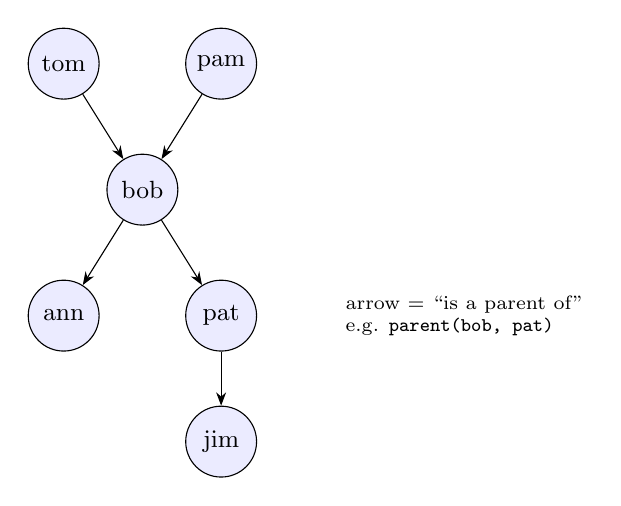
\begin{tikzpicture}[node distance=1.2cm]
\node[person](tom)at(0,0){tom};
\node[person](pam)at(2,0){pam};
\node[person](bob)at(1,-1.6){bob};
\node[person](ann)at(0,-3.2){ann};
\node[person](pat)at(2,-3.2){pat};
\node[person](jim)at(2,-4.8){jim};
\draw[->](tom)--(bob);\draw[->](pam)--(bob);
\draw[->](bob)--(ann);\draw[->](bob)--(pat);
\draw[->](pat)--(jim);
\node[font=\scriptsize,align=left,right=1cm of pat]{arrow = ``is a parent of''\\e.g. \texttt{parent(bob, pat)}};
\end{tikzpicture}
\end{center}

\subsection{Prolog Concepts Used}
\begin{itemize}[leftmargin=*]
  \item \textbf{Facts as a database} (\pred{parent/2}).
  \item \textbf{Recursion on relationships} (not on lists or numbers): an ancestor is a parent, or a parent of an ancestor.
  \item \textbf{Several clauses for one predicate}: Prolog tries them in order.
  \item \textbf{Backtracking to find all answers}: pressing \texttt{;} makes Prolog hunt for the next solution.
  \item \textbf{Intermediate variable} (\pred{Z}) linking two goals.
\end{itemize}

\subsection{Line-by-Line Explanation}
\begin{lines}
\Ln{1--5} The \pred{parent/2} facts. \pred{parent(tom, bob)} means ``tom is a parent of bob''.
\Ln{7--8} \pred{ancestor(X, Y) :- parent(X, Y).} \textbf{Base case}: a parent is an ancestor.
\Ln{9--11} \pred{ancestor(X, Y) :- parent(X, Z), ancestor(Z, Y).} \textbf{Recursive case}: \pred{X} is an ancestor of \pred{Y} if \pred{X} is a parent of some person \pred{Z}, and \pred{Z} is an ancestor of \pred{Y}. The chain is followed one generation at a time.
\Ln{13--14} \pred{descendant(X, Y) :- parent(Y, X).} \textbf{Base case}: a child is a descendant of its parent. Notice the swapped order: \pred{Y} is the parent of \pred{X}.
\Ln{15--17} \pred{descendant(X, Y) :- parent(Z, X), descendant(Z, Y).} \textbf{Recursive case}: \pred{X} is a descendant of \pred{Y} if \pred{X}'s parent \pred{Z} is a descendant of \pred{Y}.
\end{lines}

\subsection{How Prolog Works Internally}
\begin{itemize}[leftmargin=*]
  \item \textbf{Two clauses, one goal.} For any \pred{ancestor} goal Prolog first tries line 8 (direct parent). If this fails (or when you ask for more answers), it tries lines 9--11. Both kinds of answer are found.
  \item \textbf{Variable search.} In \pred{parent(X, Z)}, \pred{Z} is unbound, so Prolog scans the \pred{parent} facts from top to bottom and tries each one. If the rest of the body fails for a fact, it backtracks to the next fact. This automatic search is the heart of Prolog.
  \item \textbf{The recursion ends} because every step moves one generation down the family tree and the tree is finite. Eventually \pred{ancestor(Z, Y)} reaches either a direct \pred{parent} fact or a person with no children (failure).
  \item \textbf{Order matters.} The recursive call is placed \emph{after} \pred{parent(X, Z)}. If you wrote \pred{ancestor(Z, Y)} first (``left recursion''), Prolog would call \pred{ancestor} again with the same variables forever.
\end{itemize}

\begin{center}
\begin{tabularx}{\linewidth}{|l|X|X|}
\hline
 & \textbf{ancestor(X, Y)} & \textbf{descendant(X, Y)}\\\hline
Meaning & \pred{X} is above \pred{Y} in the tree & \pred{X} is below \pred{Y} in the tree\\\hline
Base case & \pred{parent(X, Y)} & \pred{parent(Y, X)}\\\hline
Recursive step & \pred{parent(X,Z), ancestor(Z,Y)} (go down) & \pred{parent(Z,X), descendant(Z,Y)} (go up)\\\hline
Relationship & \multicolumn{2}{X|}{\pred{descendant(A,B)} is true exactly when \pred{ancestor(B,A)} is true.}\\\hline
\end{tabularx}
\end{center}

\subsection{Step-by-Step Execution / Query Flow}
\textbf{Query 1:} \pred{?- ancestor(tom, jim).}
\begin{lstlisting}[style=tr]
ancestor(tom, jim)
  clause 1: parent(tom, jim)?  no such fact -> fail
  clause 2: parent(tom, Z)  -> first match: Z = bob
    ancestor(bob, jim)
      clause 1: parent(bob, jim)? no -> fail
      clause 2: parent(bob, Z) -> first match: Z = ann
        ancestor(ann, jim)
          clause 1: parent(ann, jim)? no
          clause 2: parent(ann, Z)? ann has no children -> fail
      backtrack: next fact parent(bob, Z) -> Z = pat
        ancestor(pat, jim)
          clause 1: parent(pat, jim)? YES
Answer: true.
\end{lstlisting}

\textbf{Query 2:} \pred{?- ancestor(X, jim).} (who are all of Jim's ancestors?) Prolog first finds \pred{X = pat} (clause 1: the fact \pred{parent(pat, jim)}). On pressing \texttt{;} it uses clause 2 and walks the facts in order: \pred{tom} (via bob, then pat), \pred{pam} (via bob, then pat), skips ann's branch (\pred{bob}-\pred{ann} leads nowhere), then \pred{bob} (via pat). Pat's own child jim leads nowhere.

\textbf{Worked example (descendants of tom).} \pred{descendant(X, tom)}: first \pred{X = bob} (direct child). Then via recursion: \pred{ann} and \pred{pat} (children of bob, who descends from tom), then \pred{jim} (child of pat).

\subsection{Sample Queries and Outputs}
\begin{lstlisting}[style=tr]
?- ancestor(tom, jim).
true.

?- ancestor(X, jim).
X = pat ;
X = tom ;
X = pam ;
X = bob.

?- descendant(X, tom).
X = bob ;
X = ann ;
X = pat ;
X = jim.

?- descendant(tom, jim).
false.
\end{lstlisting}
(The \texttt{;} after each answer is what you type to request the next one.)

\begin{keybox}
\begin{itemize}[leftmargin=*]
  \item A recursive relation = ``directly related, or related through someone who is.''
  \item Base case first and non-recursive; recursive goal \emph{last} in the body.
  \item Prolog finds all answers by backtracking; use \texttt{;} to see them.
  \item \pred{descendant} mirrors \pred{ancestor} with the \pred{parent} arguments swapped.
\end{itemize}
\end{keybox}
\begin{mnbox}
\textbf{``Parent, or parent of a parent\ldots''} (A-N-C: \textbf{A}ncestor = parent \textbf{N}ext \textbf{C}hain.)
\end{mnbox}

\newpage
% =====================================================================
\section{Simple Arithmetic Expression Evaluator}
% =====================================================================
\setcounter{subsection}{0}
\subsection{Problem Statement}
Given a term like \pred{add(3, mul(2, 4))}, evaluate the expression.

\subsection{Prolog Code}
File: \texttt{p08\_expression\_evaluator.pl}
\begin{lstlisting}[style=pl]
eval(N, N) :-                        % a plain number is its own value
    number(N).
eval(add(A, B), R) :-
    eval(A, RA),
    eval(B, RB),
    R is RA + RB.
eval(sub(A, B), R) :-
    eval(A, RA),
    eval(B, RB),
    R is RA - RB.
eval(mul(A, B), R) :-
    eval(A, RA),
    eval(B, RB),
    R is RA * RB.
eval(div(A, B), R) :-
    eval(A, RA),
    eval(B, RB),
    R is RA / RB.
\end{lstlisting}

\subsection{Prolog Concepts Used}
\begin{itemize}[leftmargin=*]
  \item \textbf{Compound terms} such as \pred{add(3, mul(2,4))}: structures with a name and arguments, which can be nested.
  \item \textbf{Pattern matching on structure}: the clause heads \pred{eval(add(A,B), R)} match only terms starting with \pred{add}.
  \item \textbf{Recursion on a tree}: evaluate both sub-expressions, then combine them.
  \item \textbf{Type test} \pred{number/1}: succeeds if its argument is a number.
  \item \textbf{\pred{is}} for the actual calculation.
\end{itemize}

An expression is a tree. Evaluating means working from the leaves (numbers) up to the root:
\begin{center}
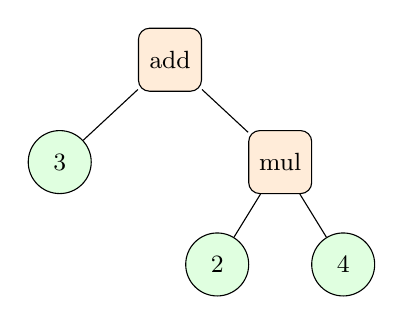
\begin{tikzpicture}[level distance=1.3cm,sibling distance=2.8cm]
\node[op]{add}
  child{node[num]{3}}
  child{node[op]{mul}
    child[sibling distance=1.6cm]{node[num]{2}}
    child[sibling distance=1.6cm]{node[num]{4}}};
\end{tikzpicture}
\end{center}

\subsection{Line-by-Line Explanation}
\begin{lines}
\Ln{1--2} \pred{eval(N, N) :- number(N).} A number evaluates to itself. The same variable \pred{N} in both positions means ``the value equals the input''. The guard \pred{number(N)} stops it matching \pred{add(...)} and the like. \textbf{Base case.}
\Ln{3--6} The \pred{add} rule: the head only matches a term shaped like \pred{add(A, B)}. Line 4 evaluates \pred{A} to \pred{RA}, line 5 evaluates \pred{B} to \pred{RB} (both are recursive calls), and line 6 adds the two results.
\Ln{7--10} The same pattern for \pred{sub} (subtraction), using \pred{-}.
\Ln{11--14} The same pattern for \pred{mul} (multiplication), using \pred{*}.
\Ln{15--18} The same pattern for \pred{div} (division), using \pred{/}.
\end{lines}

\subsection{How Prolog Works Internally}
\begin{itemize}[leftmargin=*]
  \item \textbf{Structure drives clause selection.} For \pred{eval(mul(2,4), R)}, Prolog tries clause 1: the head \pred{eval(N, N)} would bind \pred{N = mul(2,4)} and \pred{R = mul(2,4)}, but then \pred{number(N)} fails, so \emph{both bindings are undone} (backtracking). Clauses for \pred{add} and \pred{sub} do not match the name \pred{mul}. The \pred{mul} clause matches and binds \pred{A = 2}, \pred{B = 4}.
  \item \textbf{Nested expressions solve themselves.} When \pred{A} is itself an expression (like \pred{mul(2,4)}), the call \pred{eval(A, RA)} simply starts the same process again, one level deeper.
  \item \textbf{Why the arguments are evaluated before \pred{is}.} The right-hand side of \pred{is} must contain only numbers. By evaluating the parts first into \pred{RA} and \pred{RB}, which hold plain numbers, the final line is always safe.
  \item \textbf{Division.} \pred{8/4} gives the integer \pred{2}, but \pred{10/4} gives \pred{2.5}. Dividing by zero raises an error (this is a mistake in the query, not a normal \pred{false}).
\end{itemize}

\subsection{Step-by-Step Execution / Query Flow}
Query: \pred{?- eval(add(3, mul(2,4)), R).}
\begin{lstlisting}[style=tr]
eval(add(3, mul(2,4)), R)
  clause 1: N = add(...); number(add(...))? no -> undo, try next
  clause 2 (add): A = 3, B = mul(2,4)
    eval(3, RA)
      clause 1: number(3) yes -> RA = 3
    eval(mul(2,4), RB)
      clause 1: number(mul(2,4))? no
      clauses for add, sub: wrong name -> no match
      clause for mul: A = 2, B = 4
        eval(2, RA2) -> 2
        eval(4, RB2) -> 4
        R2 is 2 * 4  -> 8
      RB = 8
    R is 3 + 8 -> 11
Answer: R = 11.
\end{lstlisting}

\textbf{Worked numerical problem.} \pred{div(mul(6,4), sub(7,4))}: left side $6\times4=24$; right side $7-4=3$; result $24/3 = \mathbf{8}$.

\subsection{Sample Queries and Outputs}
\begin{lstlisting}[style=tr]
?- eval(add(3, mul(2, 4)), R).
R = 11.

?- eval(sub(10, add(2, 3)), R).
R = 5.

?- eval(div(mul(6, 4), sub(7, 4)), R).
R = 8.

?- eval(7, R).
R = 7.

?- eval(div(10, 4), R).
R = 2.5.
\end{lstlisting}

\begin{keybox}
\begin{itemize}[leftmargin=*]
  \item A nested term is a tree; recursion visits every node.
  \item Each clause head acts like a pattern for one operator.
  \item Evaluate sub-expressions first, then calculate with \pred{is}.
  \item To support a new operator, just add one more clause.
\end{itemize}
\end{keybox}
\begin{mnbox}
\textbf{``Leaves first, then climb.''} Numbers are leaves; operators combine what their children return.
\end{mnbox}

\newpage
% =====================================================================
\section{Count Occurrences of an Element}
% =====================================================================
\setcounter{subsection}{0}
\subsection{Problem Statement}
Write a predicate \pred{count_elem(List, Elem, Count)} that counts how many times \pred{Elem} appears in \pred{List}.

\subsection{Prolog Code}
File: \texttt{p09\_count\_elem.pl}
\begin{lstlisting}[style=pl]
count_elem([], _, 0).                    % nothing to count in an empty list
count_elem([E|T], E, Count) :-           % head equals the element we look for
    count_elem(T, E, Rest),
    Count is Rest + 1.
count_elem([H|T], E, Count) :-           % head is something else
    H \= E,
    count_elem(T, E, Count).
\end{lstlisting}

\subsection{Prolog Concepts Used}
\begin{itemize}[leftmargin=*]
  \item \textbf{List recursion} with three cases: empty list, head matches, head does not match.
  \item \textbf{Repeated variable in a clause head} (\pred{[E|T]} and \pred{E}): matching by unification.
  \item \textbf{\pred{\=}} (``cannot be unified'') as a guard.
  \item \textbf{Counting on the way back} with \pred{is}.
\end{itemize}

\subsection{Line-by-Line Explanation}
\begin{lines}
\Ln{1} \pred{count_elem([], _, 0).} An empty list contains the element zero times, whatever the element is (\pred{_}).
\Ln{2} \pred{count_elem([E|T], E, Count) :-} The \emph{same} variable \pred{E} is used for the head of the list and for the second argument. This clause therefore applies only when the head \textbf{equals} the element we are counting.
\Ln{3} \pred{count_elem(T, E, Rest),} Count the occurrences in the tail.
\Ln{4} \pred{Count is Rest + 1.} The head was a match, so add one.
\Ln{5} \pred{count_elem([H|T], E, Count) :-} Case where the head may be something else.
\Ln{6} \pred{H \= E,} Guard: \pred{H} and \pred{E} are different, so this head does not count.
\Ln{7} \pred{count_elem(T, E, Count).} Skip the head; the count of the whole list equals the count of the tail.
\end{lines}

\subsection{How Prolog Works Internally}
\begin{itemize}[leftmargin=*]
  \item \textbf{Repeated variables mean ``must be equal''.} To match the goal \pred{count_elem([b,a], a, C)} with line 2's head, Prolog binds \pred{E} to the first argument's head \pred{b}, then must unify \pred{E} with the second argument \pred{a}. Since \pred{b} and \pred{a} differ, unification fails and line 2 is rejected \emph{before} its body starts.
  \item Prolog then moves to line 5, whose guard \pred{b \= a} is true, so it skips the head.
  \item If the head does match (for \pred{[a,...]} and \pred{a}), line 2 applies. Line 5 would also unify with the head, but its guard \pred{a \= a} fails, so no duplicate answer is produced.
  \item The base case (line 1) stops the recursion once the list is empty.
\end{itemize}

\begin{center}
\begin{tabularx}{\linewidth}{|l|X|X|}
\hline
\textbf{Operator} & \textbf{Meaning} & \textbf{Typical use}\\\hline
\pred{=} / \pred{\=} & Unifies / cannot unify (works on any terms) & Comparing atoms and lists, as in this problem\\\hline
\pred{=:=} / \pred{=\=} & Equal / not equal \emph{as numbers} (needs numbers) & Arithmetic tests such as \pred{H mod 2 =:= 0}\\\hline
\end{tabularx}
\end{center}

\subsection{Step-by-Step Execution / Query Flow}
Query: \pred{?- count_elem([a,b,a], a, C).}
\begin{lstlisting}[style=tr]
count_elem([a,b,a], a, C)
  clause 2: E = a (from head) and E = a (2nd arg) -> match; T = [b,a]
    count_elem([b,a], a, Rest)
      clause 2: E = b vs a -> mismatch, rejected
      clause 3: H = b; b \= a true; T = [a]
        count_elem([a], a, Rest2)
          clause 2: match; T = []
            count_elem([], a, Rest3) -> clause 1: Rest3 = 0
            Count2 is 0 + 1 -> 1
      (clause 3 returns the same value) Rest = 1
    Count is 1 + 1 -> 2
Answer: C = 2.
\end{lstlisting}

\textbf{Worked numerical problem.} \pred{count_elem([a,b,a,c,a], a, C)}: positions 1, 3, 5 match; the answer is $1+1+1 = \mathbf{3}$.

\subsection{Sample Queries and Outputs}
\begin{lstlisting}[style=tr]
?- count_elem([a,b,a,c,a], a, C).
C = 3.

?- count_elem([a,b,c], z, C).
C = 0.

?- count_elem([], a, C).
C = 0.

?- count_elem([1,2,1,1], 1, 3).
true.
\end{lstlisting}

\begin{keybox}
\begin{itemize}[leftmargin=*]
  \item Using one variable in two places of a clause head forces equality.
  \item \pred{\=} is the opposite test: ``cannot be made equal''.
  \item Two competing clauses should have conditions that exclude each other.
\end{itemize}
\end{keybox}
\begin{mnbox}
\textbf{``Match: plus one. Miss: pass on.''}
\end{mnbox}

\newpage
% =====================================================================
\section{Find All Siblings}
% =====================================================================
\setcounter{subsection}{0}
\subsection{Problem Statement}
Given \pred{parent/2} facts, write a rule to find all siblings of a person using \pred{findall/3}.

\subsection{Prolog Code}
File: \texttt{p10\_find\_siblings.pl}
\begin{lstlisting}[style=pl]
parent(tom, bob).
parent(pam, bob).
parent(tom, liz).
parent(pam, liz).
parent(tom, jack).
parent(pam, jack).
parent(bob, ann).
parent(bob, pat).

sibling(X, Y) :-                     % same parent, but not the same person
    parent(P, X),
    parent(P, Y),
    X \= Y.

find_siblings(Person, Siblings) :-
    findall(S, sibling(Person, S), AllSiblings),
    sort(AllSiblings, Siblings).     % sort also removes duplicates
\end{lstlisting}

The family used in the facts (arrows mean ``is a parent of''):
\begin{center}
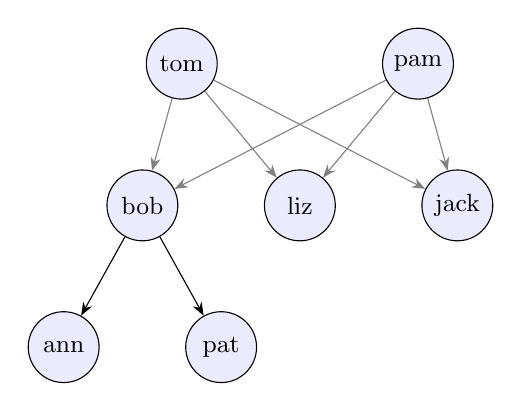
\begin{tikzpicture}
\node[person](tom)at(0.5,0){tom};
\node[person](pam)at(3.5,0){pam};
\node[person](bob)at(0,-1.8){bob};
\node[person](liz)at(2,-1.8){liz};
\node[person](jack)at(4,-1.8){jack};
\node[person](ann)at(-1,-3.6){ann};
\node[person](pat)at(1,-3.6){pat};
\foreach \p in {tom,pam}{\foreach \c in {bob,liz,jack}{\draw[->,gray](\p)--(\c);}}
\draw[->](bob)--(ann);\draw[->](bob)--(pat);
\end{tikzpicture}
\end{center}

\subsection{Prolog Concepts Used}
\begin{itemize}[leftmargin=*]
  \item \textbf{Rule with a shared variable}: \pred{P} links the two \pred{parent} goals (same parent).
  \item \textbf{\pred{\=}} to exclude the person himself or herself.
  \item \textbf{\pred{findall/3}}: collects every solution of a goal in a list.
  \item \textbf{\pred{sort/2}}: orders a list and removes duplicates.
  \item \textbf{Backtracking}: \pred{findall} makes Prolog explore all possibilities.
\end{itemize}

\subsection{Line-by-Line Explanation}
\begin{lines}
\Ln{1--8} The \pred{parent/2} facts. Tom and Pam are the parents of Bob, Liz and Jack; Bob is the parent of Ann and Pat.
\Ln{10} \pred{sibling(X, Y) :-} ``\pred{X} and \pred{Y} are siblings if\ldots''
\Ln{11} \pred{parent(P, X),} \ldots some \pred{P} is a parent of \pred{X}, and
\Ln{12} \pred{parent(P, Y),} \ldots the \emph{same} \pred{P} is a parent of \pred{Y}, and
\Ln{13} \pred{X \= Y.} \ldots \pred{X} and \pred{Y} are not the same person (otherwise everybody would be their own sibling).
\Ln{15} \pred{find_siblings(Person, Siblings) :-} The predicate asked for in the problem.
\Ln{16} \pred{findall(S, sibling(Person, S), AllSiblings),} Collect every value of \pred{S} for which \pred{sibling(Person, S)} holds, into the list \pred{AllSiblings}.
\Ln{17} \pred{sort(AllSiblings, Siblings).} Remove duplicates (and sort alphabetically) to produce the final list.
\end{lines}

\subsection{How Prolog Works Internally}
\begin{itemize}[leftmargin=*]
  \item \textbf{How \pred{findall} works.} Prolog runs the goal. Every time it succeeds, \pred{findall} copies the template value (\pred{S}) into a result list, then \emph{deliberately forces a failure} so that Prolog backtracks and finds the next solution. When no solutions remain, the list is complete and returned. If there were no solutions at all, the result is \pred{[]}.
  \item \textbf{Why duplicates appear.} In this family, Bob and Liz share \emph{two} parents. The sibling relationship is proved once through \pred{P = tom} and once through \pred{P = pam}. So \pred{findall} finds \pred{liz} twice (and \pred{jack} twice).
  \item \textbf{Why \pred{sort/2} is used.} It removes these repeated entries, giving each sibling exactly once.
  \item \textbf{Why \pred{\=} is on the last line.} By the time it runs, both \pred{X} and \pred{Y} have values, so the test is meaningful. Placed earlier, with \pred{Y} still unbound, it would not work as intended.
  \item Someone with no recorded parents (tom) has no siblings by this definition, and \pred{findall} returns \pred{[]}.
\end{itemize}

\subsection{Step-by-Step Execution / Query Flow}
Query: \pred{?- find_siblings(bob, L).}  \quad Prolog first runs \pred{findall(S, sibling(bob, S), All)}:
\begin{lstlisting}[style=tr]
sibling(bob, S):
  parent(P, bob)            -> first match: P = tom
    parent(tom, Y)          tries each fact whose first argument is tom:
      Y = bob   -> bob \= bob fails            (not collected)
      Y = liz   -> bob \= liz ok -> S = liz    COLLECT liz
      Y = jack  -> ok            -> S = jack   COLLECT jack
  backtrack: parent(P, bob) -> next match: P = pam
    parent(pam, Y)
      Y = bob   -> fails
      Y = liz   -> COLLECT liz
      Y = jack  -> COLLECT jack
  no more parents of bob.
All = [liz, jack, liz, jack]
\end{lstlisting}
Then \pred{sort(All, Siblings)} removes duplicates and sorts: \pred{Siblings = [jack, liz]}.

\textbf{Worked example.} Siblings of \pred{ann}: her parent is bob; bob's other child is \pred{pat} (\pred{ann} herself is excluded by \pred{\=}). Result \pred{[pat]}.

\subsection{Sample Queries and Outputs}
\begin{lstlisting}[style=tr]
?- find_siblings(bob, L).
L = [jack, liz].

?- findall(S, sibling(bob, S), L).     % without sort: duplicates remain
L = [liz, jack, liz, jack].

?- find_siblings(ann, L).
L = [pat].

?- find_siblings(tom, L).              % no parent facts for tom
L = [].
\end{lstlisting}

\begin{keybox}
\begin{itemize}[leftmargin=*]
  \item \pred{findall(Template, Goal, List)} = ``give me all solutions of Goal as a list''.
  \item Use \pred{\=} to exclude the person from his or her own siblings.
  \item Use \pred{sort/2} to remove duplicates produced when a relationship can be proved in several ways.
  \item \pred{findall} never fails: no solutions simply give \pred{[]}.
\end{itemize}
\end{keybox}
\begin{mnbox}
\textbf{``Same parent, different person.''} Sibling = \emph{S}hared parent + \emph{D}ifferent child (S-D). And: \textbf{findall = find ALL.}
\end{mnbox}

\newpage

% =====================================================================
\section{N-th Element of a List}
% =====================================================================
\setcounter{subsection}{0}
\subsection{Problem Statement}
Write a predicate \pred{nth_element(N, List, Elem)} that retrieves the N-th element of a list (1-based indexing: the first element is number 1).

\subsection{Prolog Code}
File: \texttt{p11\_nth\_element.pl}
\begin{lstlisting}[style=pl]
nth_element(1, [H|_], H).                % the 1st element is the head
nth_element(N, [_|T], Elem) :-
    N > 1,
    N1 is N - 1,                         % one step closer to the front
    nth_element(N1, T, Elem).            % ask the same question about the tail
\end{lstlisting}

\subsection{Prolog Concepts Used}
\begin{itemize}[leftmargin=*]
  \item \textbf{Recursion on a counter and a list at the same time}: the number goes down while the list gets shorter.
  \item \textbf{Patterns} \pred{[H|_]} (take the head) and \pred{[_|T]} (discard the head).
  \item \textbf{Arithmetic} with \pred{is} and a guard with \pred{>}.
  \item \textbf{Failure as an answer}: asking for a position that does not exist simply fails.
\end{itemize}

\subsection{Line-by-Line Explanation}
\begin{lines}
\Ln{1} \pred{nth_element(1, [H|_], H).} Base case: the 1st element of a list is its head. The same variable \pred{H} in the list pattern and in the third position means \pred{Elem} is the head.
\Ln{2} \pred{nth_element(N, [_|T], Elem) :-} Recursive case: throw away the head (\pred{_}) and keep the tail \pred{T}.
\Ln{3} \pred{N > 1,} Guard: only recurse if we have not yet reached position 1. This also rejects 0 and negative positions.
\Ln{4} \pred{N1 is N - 1,} After removing one element, the wanted element is one position earlier.
\Ln{5} \pred{nth_element(N1, T, Elem).} Ask the same question on the shorter list with the smaller number. The answer \pred{Elem} is passed straight through.
\end{lines}

\subsection{How Prolog Works Internally}
\begin{itemize}[leftmargin=*]
  \item For \pred{nth_element(3, [a,b,c,d], E)}, line 1 is tried first. Its first argument is the number \pred{1}, which does not unify with \pred{3}, so it is rejected immediately. Line 2 matches.
  \item Every recursive call removes the head and decrements \pred{N}. When the counter reaches \pred{1}, line 1 matches and \pred{Elem} receives the head of whatever list remains.
  \item \textbf{The answer needs no calculation on the way back}: \pred{Elem} is the same variable all the way down, and it is bound at the bottom.
  \item \textbf{Out of range.} For \pred{nth_element(5, [a,b], E)} the list shrinks to \pred{[]} while \pred{N} is still bigger than 1. Neither clause matches \pred{[]} (both need a head), so the goal fails and Prolog answers \pred{false}.
  \item \textbf{Limitation.} The guard \pred{N > 1} needs \pred{N} to have a numeric value. Asking \pred{nth_element(N, [a,b,c], c)} (``where is c?'') raises an error because \pred{N} is unbound.
\end{itemize}

\subsection{Step-by-Step Execution / Query Flow}
Query: \pred{?- nth_element(3, [a,b,c,d], E).}
\begin{lstlisting}[style=tr]
nth_element(3, [a,b,c,d], E)
  clause 1: 1 vs 3 -> no match
  clause 2: N = 3, T = [b,c,d]
    3 > 1 -> true;  N1 is 3 - 1 -> 2
    nth_element(2, [b,c,d], E)
      clause 1: 1 vs 2 -> no match
      clause 2: N = 2, T = [c,d]
        2 > 1 -> true;  N1 is 2 - 1 -> 1
        nth_element(1, [c,d], E)
          clause 1: 1 = 1 ok; [H|_] = [c,d] -> H = c; E = c
Answer: E = c.
\end{lstlisting}

\textbf{Worked numerical problem.} 4th element of \pred{[10,20,30,40,50]}: remove 10 (now position 3), remove 20 (position 2), remove 30 (position 1): the head is \textbf{40}.

\subsection{Sample Queries and Outputs}
\begin{lstlisting}[style=tr]
?- nth_element(3, [a,b,c,d], E).
E = c.

?- nth_element(1, [x,y], E).
E = x.

?- nth_element(4, [10,20,30,40,50], E).
E = 40.

?- nth_element(5, [a,b], E).
false.

?- nth_element(0, [a,b], E).
false.
\end{lstlisting}

\begin{keybox}
\begin{itemize}[leftmargin=*]
  \item Count down while walking down the list: position $N$ in a list is position $N-1$ in its tail.
  \item The base case position is 1 (1-based indexing).
  \item A guard \pred{N > 1} avoids endless searching and rejects invalid positions.
  \item Running off the end of the list leads to failure, not to an error.
\end{itemize}
\end{keybox}
\begin{mnbox}
\textbf{``Drop one, count one.''} Every time you discard a head, lower the counter by one.
\end{mnbox}

\newpage
% =====================================================================
\section{Check if List is Sorted}
% =====================================================================
\setcounter{subsection}{0}
\subsection{Problem Statement}
Write a predicate \pred{sorted(List)} that succeeds only if the list is sorted in ascending order.

\subsection{Prolog Code}
File: \texttt{p12\_sorted.pl}
\begin{lstlisting}[style=pl]
sorted([]).                          % empty list is sorted
sorted([_]).                         % one element is sorted
sorted([X, Y|T]) :-                  % compare the first two elements
    X =< Y,
    sorted([Y|T]).                   % then check the rest
\end{lstlisting}

\subsection{Prolog Concepts Used}
\begin{itemize}[leftmargin=*]
  \item \textbf{Looking at two elements at once} with the pattern \pred{[X, Y|T]}.
  \item \textbf{Multiple base cases} (empty list and single-element list).
  \item \textbf{Arithmetic comparison} \pred{=<}.
  \item \textbf{Predicates that only answer yes or no} (no output variable).
\end{itemize}

\subsection{Line-by-Line Explanation}
\begin{lines}
\Ln{1} \pred{sorted([]).} An empty list is sorted (nothing can be out of order).
\Ln{2} \pred{sorted([_]).} A one-element list is sorted. The element's value is irrelevant, so we use \pred{_}.
\Ln{3} \pred{sorted([X, Y|T]) :-} A list with at least two elements: first element \pred{X}, second \pred{Y}, everything after is \pred{T}.
\Ln{4} \pred{X =< Y,} The first two elements must be in order. (\pred{=<} allows equal values, so \pred{[2,2]} counts as sorted.)
\Ln{5} \pred{sorted([Y|T]).} Check the rest of the list, starting from \pred{Y}. Because \pred{Y} is kept as the new first element, the next comparison is \pred{Y} versus the element after it. Every neighbouring pair gets checked.
\end{lines}

\subsection{How Prolog Works Internally}
\begin{itemize}[leftmargin=*]
  \item \textbf{Why line 2 is needed.} The pattern \pred{[X, Y|T]} requires \emph{two} elements. Without line 2, the final one-element list \pred{[5]} would match no clause and the whole check would fail even for a perfectly sorted list.
  \item \textbf{Early exit on failure.} As soon as one pair is out of order, \pred{X =< Y} fails. No other clause can rescue it (a list with two or more elements only matches line 3), so Prolog answers \pred{false} immediately without looking at the rest.
  \item \textbf{Rebuilding the list.} \pred{[Y|T]} on line 5 builds a fresh list by attaching \pred{Y} in front of \pred{T}. This effectively moves the ``window'' of two elements forward by one position.
  \item Each call works on a list that is one element shorter, so the recursion ends at line 2.
\end{itemize}

\subsection{Step-by-Step Execution / Query Flow}
\textbf{Success:} \pred{?- sorted([1,2,5]).}
\begin{lstlisting}[style=tr]
sorted([1,2,5])
  clause 3: X=1, Y=2, T=[5];  1 =< 2 true
  sorted([2,5])
    clause 3: X=2, Y=5, T=[];  2 =< 5 true
    sorted([5])
      clause 2 matches [_]  -> true
Answer: true.
\end{lstlisting}
\textbf{Failure:} \pred{?- sorted([1,3,2]).}
\begin{lstlisting}[style=tr]
sorted([1,3,2])
  clause 3: X=1, Y=3, T=[2];  1 =< 3 true
  sorted([3,2])
    clause 3: X=3, Y=2, T=[];  3 =< 2 FALSE -> fail
    no other clause matches a 2-element list
Answer: false.
\end{lstlisting}

\begin{center}
\begin{tabularx}{\linewidth}{|l|X|X|}
\hline
\textbf{List} & \textbf{Pairs compared} & \textbf{Result}\\\hline
\pred{[1,2,2,5,9]} & $1\le2,\ 2\le2,\ 2\le5,\ 5\le9$ & true\\\hline
\pred{[4,6,3]} & $4\le6$ ok, $6\le3$ fails & false\\\hline
\pred{[7]} & none & true\\\hline
\end{tabularx}
\end{center}

\subsection{Sample Queries and Outputs}
\begin{lstlisting}[style=tr]
?- sorted([1,2,2,5,9]).
true.

?- sorted([1,3,2]).
false.

?- sorted([]).
true.

?- sorted([7]).
true.
\end{lstlisting}

\begin{keybox}
\begin{itemize}[leftmargin=*]
  \item A list is sorted if \emph{every pair of neighbours} is in order.
  \item The pattern \pred{[X, Y|T]} peeks at two elements; pass \pred{[Y|T]} on.
  \item Provide base cases for both the empty list and the one-element list.
  \item For a duplicates-not-allowed check, change \pred{=<} to \pred{<}.
\end{itemize}
\end{keybox}
\begin{mnbox}
\textbf{``Each neighbour pair must be fair.''} (Left $\le$ right, all the way down.)
\end{mnbox}

\newpage
% =====================================================================
\section{Check Prime Number}
% =====================================================================
\setcounter{subsection}{0}
\subsection{Problem Statement}
Define \pred{is_prime(N)} that checks if \pred{N} is a prime using basic divisor checking.

\begin{defbox}{Prime number}
A prime is a whole number greater than 1 whose only divisors are 1 and itself. Examples: 2, 3, 5, 7, 11. Non-examples: 1 (not greater than 1), 4 ($=2\times2$), 9 ($=3\times3$).
\end{defbox}

\subsection{Prolog Code}
File: \texttt{p13\_is\_prime.pl}
\begin{lstlisting}[style=pl]
is_prime(N) :-
    N > 1,                           % 0, 1 and negatives are not prime
    \+ has_divisor(N, 2).            % no divisor found, starting from 2

has_divisor(N, D) :-                 % D divides N exactly
    D * D =< N,
    N mod D =:= 0.
has_divisor(N, D) :-                 % otherwise try the next D
    D * D =< N,
    D1 is D + 1,
    has_divisor(N, D1).
\end{lstlisting}

\subsection{Prolog Concepts Used}
\begin{itemize}[leftmargin=*]
  \item \textbf{Negation as failure} (\pred{\+}): ``there is no divisor''.
  \item \textbf{Helper predicate} that searches for a divisor.
  \item \textbf{Counting upwards} (\pred{D1 is D + 1}) in a recursive search.
  \item \textbf{\pred{mod}} and \pred{=:=} to test divisibility.
  \item \textbf{Stopping condition} \pred{D * D =< N}: only try divisors up to the square root of \pred{N}.
\end{itemize}

\subsection{Line-by-Line Explanation}
\begin{lines}
\Ln{1} \pred{is_prime(N) :-} ``\pred{N} is prime if\ldots''
\Ln{2} \pred{N > 1,} \ldots it is greater than 1 (this rules out 1, 0 and negative numbers), and
\Ln{3} \pred{\+ has_divisor(N, 2).} \ldots it is \emph{not} the case that some divisor exists, starting the search at 2.
\Ln{4} \pred{has_divisor(N, D) :-} ``\pred{N} has a divisor, starting the search from \pred{D}, if\ldots''
\Ln{5} \pred{D * D =< N,} \ldots \pred{D} has not gone past the square root of \pred{N}, and
\Ln{6} \pred{N mod D =:= 0.} \ldots \pred{D} divides \pred{N} exactly (remainder 0). \textbf{Found a divisor.}
\Ln{7} \pred{has_divisor(N, D) :-} Second way to have a divisor: it is found further on.
\Ln{8} \pred{D * D =< N,} We are still within the square-root limit.
\Ln{9} \pred{D1 is D + 1,} Move to the next candidate divisor.
\Ln{10} \pred{has_divisor(N, D1).} Keep searching with the next candidate.
\end{lines}

\subsection{How Prolog Works Internally}
\begin{itemize}[leftmargin=*]
  \item \textbf{How \pred{\+} works.} Prolog runs \pred{has_divisor(N, 2)}. If this \emph{succeeds}, \pred{\+} fails (so \pred{is_prime} fails: not prime). If it \emph{fails} after trying everything, \pred{\+} succeeds (prime). Variable bindings made inside a \pred{\+} are never kept.
  \item \textbf{Why only up to the square root.} If $N = a \times b$, at least one of $a,b$ is $\le \sqrt N$. So if no divisor exists up to $\sqrt N$, none exists at all. The test $D \times D \le N$ is the same as $D \le \sqrt N$ but uses only whole-number arithmetic.
  \item \textbf{Two clauses, one search.} Clause 1 (line 4) succeeds when \pred{D} divides \pred{N}. If it fails, Prolog backtracks into clause 2 (line 7), which tries \pred{D+1}. When $D \times D > N$, \emph{both} clauses fail at their first goal, which means ``no divisor found'' and the search ends with failure.
  \item The recursion terminates because \pred{D} grows by 1 each time while \pred{N} stays fixed, so \pred{D * D} eventually exceeds \pred{N}.
\end{itemize}

\begin{center}
\begin{tabularx}{\linewidth}{|l|X|X|}
\hline
\textbf{N} & \textbf{What the search does} & \textbf{Result}\\\hline
1 & fails \pred{N > 1} at once & not prime\\\hline
2 & $2\times2=4>2$: no divisor candidates & prime\\\hline
4 & $D=2$: $4 \bmod 2 = 0$, divisor found & not prime\\\hline
9 & $D=2$: remainder 1; $D=3$: $9 \bmod 3=0$ & not prime\\\hline
7 & $D=2$: remainder 1; $D=3$: $9>7$, stop & prime\\\hline
\end{tabularx}
\end{center}

\subsection{Step-by-Step Execution / Query Flow}
Query: \pred{?- is_prime(7).}
\begin{lstlisting}[style=tr]
is_prime(7)
  7 > 1 -> true
  \+ has_divisor(7, 2)   (prove has_divisor(7,2); \+ succeeds only if it fails)
    has_divisor(7, 2):
      clause 1: 2*2 = 4 =< 7 true;  7 mod 2 = 1, 1 =:= 0 false -> fail
      clause 2: 4 =< 7 true;  D1 = 3
        has_divisor(7, 3):
          clause 1: 3*3 = 9 =< 7 false -> fail
          clause 2: 9 =< 7 false -> fail
        fails
      fails
    has_divisor failed everywhere -> \+ succeeds
Answer: true.
\end{lstlisting}
Query: \pred{?- is_prime(15).}
\begin{lstlisting}[style=tr]
has_divisor(15, 2): 4 =< 15, 15 mod 2 = 1 -> clause 1 fails
  clause 2: D1 = 3 -> has_divisor(15, 3):
    clause 1: 9 =< 15 true;  15 mod 3 = 0 true -> SUCCESS (divisor 3 found)
\+ has_divisor(...) therefore fails -> is_prime(15) fails.
Answer: false.
\end{lstlisting}

\textbf{Worked numerical problem.} Is 29 prime? $D=2,3,4,5$ are tested ($4,9,16,25 \le 29$): $29 \bmod 2=1$, $29 \bmod 3=2$, $29 \bmod 4=1$, $29 \bmod 5=4$, none is 0. Then $D=6$: $36>29$, so the search stops: \textbf{29 is prime}.

\subsection{Sample Queries and Outputs}
\begin{lstlisting}[style=tr]
?- is_prime(7).
true.

?- is_prime(15).
false.

?- is_prime(2).
true.

?- is_prime(1).
false.

?- is_prime(29).
true.
\end{lstlisting}

\begin{keybox}
\begin{itemize}[leftmargin=*]
  \item \pred{\+ Goal} succeeds exactly when \pred{Goal} cannot be proved.
  \item A helper that counts upward (\pred{D}, \pred{D+1}, \dots) searches for a divisor.
  \item $D \times D \le N$ is a cheap way to stop at the square root.
  \item \pred{is_prime} needs a number given as input; it is not designed to generate primes.
\end{itemize}
\end{keybox}
\begin{mnbox}
\textbf{``Prime = no divisor up to the root.''} (P-R-D: \textbf{P}rime \textbf{R}ejects any \textbf{D}ivisor.)
\end{mnbox}

\newpage
% =====================================================================
\section{Fibonacci Series Generator (Non-memoized)}
% =====================================================================
\setcounter{subsection}{0}
\subsection{Problem Statement}
Write a predicate \pred{fib(N, F)} to generate the N-th Fibonacci number recursively.

\begin{defbox}{Fibonacci numbers}
$F_0 = 0,\quad F_1 = 1,\quad F_n = F_{n-1} + F_{n-2}\ (n\ge2)$.\\
The sequence is $0, 1, 1, 2, 3, 5, 8, 13, 21, 34, 55, \dots$
\end{defbox}

\subsection{Prolog Code}
File: \texttt{p14\_fibonacci.pl}
\begin{lstlisting}[style=pl]
fib(0, 0).                           % base case 1
fib(1, 1).                           % base case 2
fib(N, F) :-
    N > 1,
    N1 is N - 1,
    N2 is N - 2,
    fib(N1, F1),
    fib(N2, F2),
    F is F1 + F2.
\end{lstlisting}

\subsection{Prolog Concepts Used}
\begin{itemize}[leftmargin=*]
  \item \textbf{Two base cases} (\pred{fib(0,0)} and \pred{fib(1,1)}).
  \item \textbf{Two recursive calls} in one rule (\emph{tree recursion}).
  \item \textbf{Intermediate variables} \pred{N1}, \pred{N2}, \pred{F1}, \pred{F2}.
  \item \textbf{Guard} \pred{N > 1} to keep the recursive clause away from the base cases.
\end{itemize}

\subsection{Line-by-Line Explanation}
\begin{lines}
\Ln{1} \pred{fib(0, 0).} Base case: the 0th Fibonacci number is 0.
\Ln{2} \pred{fib(1, 1).} Base case: the 1st Fibonacci number is 1.
\Ln{3} \pred{fib(N, F) :-} Recursive rule for all larger \pred{N}.
\Ln{4} \pred{N > 1,} Guard: this rule applies only when \pred{N} is at least 2.
\Ln{5} \pred{N1 is N - 1,} Position just before \pred{N}.
\Ln{6} \pred{N2 is N - 2,} Position two before \pred{N}.
\Ln{7} \pred{fib(N1, F1),} Compute $F_{n-1}$ recursively.
\Ln{8} \pred{fib(N2, F2),} Compute $F_{n-2}$ recursively.
\Ln{9} \pred{F is F1 + F2.} The answer is their sum.
\end{lines}

\subsection{How Prolog Works Internally}
\begin{itemize}[leftmargin=*]
  \item \textbf{Tree-shaped execution.} The body has \emph{two} recursive goals, so each call spawns two more calls. Prolog finishes line 7 completely (the whole left subtree) before starting line 8.
  \item \textbf{Fresh variables everywhere.} Each call has its own \pred{N1}, \pred{N2}, \pred{F1}, \pred{F2}, so the many simultaneous calls never interfere.
  \item \textbf{Why the guard.} For \pred{fib(1, F)}, line 2 gives \pred{F = 1}. The head of line 3 would also unify, but \pred{1 > 1} fails, so no wrong second answer appears. Without the guard, the program would also recurse into negative numbers forever.
  \item \textbf{``Non-memoized'' means repeated work.} Prolog does not remember results it already computed. In the picture below, \pred{fib(2)} is calculated twice, and \pred{fib(1)} three times, even when computing only \pred{fib(4)}.
\end{itemize}

\begin{center}
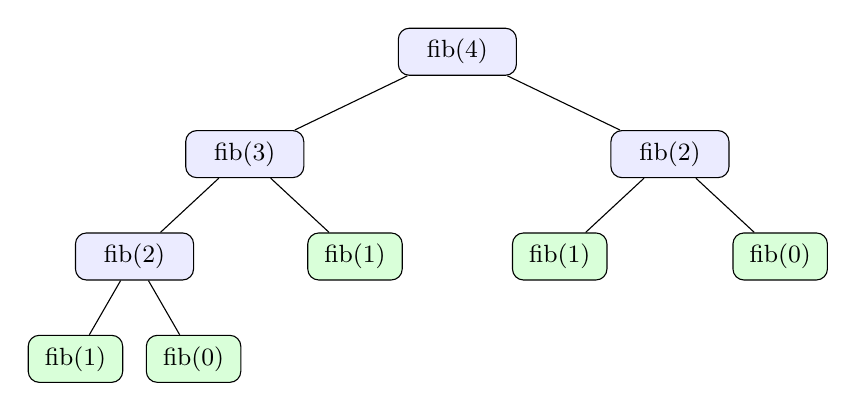
\begin{tikzpicture}[level distance=1.3cm,
  level 1/.style={sibling distance=5.4cm},
  level 2/.style={sibling distance=2.8cm},
  level 3/.style={sibling distance=1.5cm},
  every node/.style={font=\footnotesize,inner sep=3pt}]
\node[box,minimum width=1.5cm]{fib(4)}
  child{node[box,minimum width=1.5cm]{fib(3)}
    child{node[box,minimum width=1.5cm]{fib(2)}
      child{node[good,minimum width=1.2cm]{fib(1)}}
      child{node[good,minimum width=1.2cm]{fib(0)}}}
    child{node[good,minimum width=1.2cm]{fib(1)}}}
  child{node[box,minimum width=1.5cm]{fib(2)}
    child{node[good,minimum width=1.2cm]{fib(1)}}
    child{node[good,minimum width=1.2cm]{fib(0)}}};
\end{tikzpicture}

\footnotesize Green nodes are base cases. Results: fib(1)=1, fib(0)=0, fib(2)=1, fib(3)=2, fib(4)=3.
\end{center}

\begin{center}
\begin{tabularx}{\linewidth}{|X|X|}
\hline
\textbf{Computing} & \textbf{Number of calls to \pred{fib}}\\\hline
\pred{fib(5)} & 15\\\hline
\pred{fib(10)} & 177\\\hline
\pred{fib(20)} & 21\,891\\\hline
\pred{fib(30)} & 2\,692\,537\\\hline
\end{tabularx}
\end{center}
The number of calls roughly multiplies by 1.6 for each step in \pred{N}. This is why this simple definition becomes very slow for large \pred{N} (try \pred{fib(35, F)} and \pred{fib(40, F)} to feel it). It is, however, the simplest and clearest definition, which is what the problem asks for.

\subsection{Step-by-Step Execution / Query Flow}
Query: \pred{?- fib(4, F).}
\begin{lstlisting}[style=tr]
fib(4, F)
  clause 3: N = 4; 4 > 1; N1 = 3; N2 = 2
  fib(3, F1)
    N = 3; N1 = 2; N2 = 1
    fib(2, Fa)
      N = 2; N1 = 1; N2 = 0
      fib(1, Fb)  -> clause 2: Fb = 1
      fib(0, Fc)  -> clause 1: Fc = 0
      Fa is 1 + 0 -> 1
    fib(1, Fd)    -> clause 2: Fd = 1
    F1 is 1 + 1   -> 2
  fib(2, F2)
    N1 = 1; N2 = 0
    fib(1, ...) -> 1;  fib(0, ...) -> 0
    F2 is 1 + 0   -> 1
  F is 2 + 1      -> 3
Answer: F = 3.
\end{lstlisting}

\textbf{Worked numerical problem.} Build the sequence bottom-up to check: $F_2=1+0=1$, $F_3=1+1=2$, $F_4=2+1=3$, $F_5=3+2=5$, $F_6=5+3=8$, $F_7=8+5=\mathbf{13}$.

\subsection{Sample Queries and Outputs}
\begin{lstlisting}[style=tr]
?- fib(0, F).
F = 0.

?- fib(1, F).
F = 1.

?- fib(5, F).
F = 5.

?- fib(7, F).
F = 13.

?- fib(10, F).
F = 55.
\end{lstlisting}

\begin{keybox}
\begin{itemize}[leftmargin=*]
  \item Two base cases for the first two terms; one recursive rule for the rest.
  \item Two recursive calls give a call \emph{tree}, not a single chain.
  \item Without memoization the same sub-problems are recomputed, which is simple but slow for large \pred{N}.
  \item Always keep the guard \pred{N > 1} so that the rules do not overlap.
\end{itemize}
\end{keybox}
\begin{mnbox}
\textbf{``Each number is the sum of the previous two''}: 0, 1, then add the last two.
\end{mnbox}

\newpage
% =====================================================================
\section{Family Tree -- Uncle/Aunt Relation}
% =====================================================================
\setcounter{subsection}{0}
\subsection{Problem Statement}
Extend \pred{parent/2} to define \pred{uncle/2} or \pred{aunt/2} using \pred{sibling/2}. (This solution defines \emph{both}.)

\subsection{Prolog Code}
File: \texttt{p15\_uncle\_aunt.pl}
\begin{lstlisting}[style=pl]
parent(tom, bob).
parent(tom, liz).
parent(bob, ann).
parent(bob, pat).
parent(liz, sue).

male(tom).
male(bob).
male(pat).
female(liz).
female(ann).
female(sue).

sibling(X, Y) :-
    parent(P, X),
    parent(P, Y),
    X \= Y.

uncle(U, Child) :-                   % U is a male sibling of Child's parent
    parent(P, Child),
    sibling(U, P),
    male(U).

aunt(A, Child) :-                    % A is a female sibling of Child's parent
    parent(P, Child),
    sibling(A, P),
    female(A).
\end{lstlisting}

The family (arrows mean ``is a parent of''; blue = male, pink = female):
\begin{center}
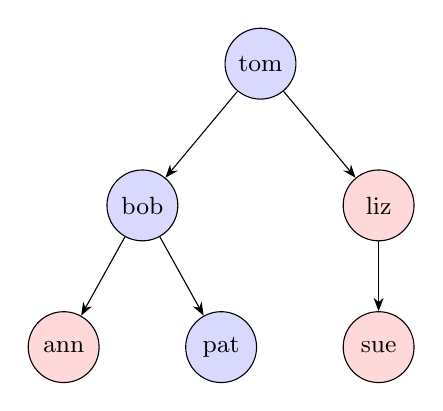
\begin{tikzpicture}
\tikzset{m/.style={person,fill=blue!15},f/.style={person,fill=pink!60}}
\node[m](tom)at(1,0){tom};
\node[m](bob)at(-0.5,-1.8){bob};
\node[f](liz)at(2.5,-1.8){liz};
\node[f](ann)at(-1.5,-3.6){ann};
\node[m](pat)at(0.5,-3.6){pat};
\node[f](sue)at(2.5,-3.6){sue};
\draw[->](tom)--(bob);\draw[->](tom)--(liz);
\draw[->](bob)--(ann);\draw[->](bob)--(pat);
\draw[->](liz)--(sue);
\end{tikzpicture}
\end{center}

\subsection{Prolog Concepts Used}
\begin{itemize}[leftmargin=*]
  \item \textbf{Facts} for parents and genders (\pred{male/1}, \pred{female/1}).
  \item \textbf{Building new relations from old ones}: \pred{uncle} uses \pred{parent} and \pred{sibling}.
  \item \textbf{A rule with several goals} joined by \pred{,} (AND).
  \item \textbf{Variables as connectors} between goals (\pred{P}).
  \item \textbf{Filtering with a fact} (\pred{male(U)}) after finding candidates.
\end{itemize}

\subsection{Line-by-Line Explanation}
\begin{lines}
\Ln{1--5} The \pred{parent/2} facts. Tom is the parent of Bob and Liz; Bob of Ann and Pat; Liz of Sue.
\Ln{7--12} The gender facts: \pred{male/1} for tom, bob, pat; \pred{female/1} for liz, ann, sue.
\Ln{14--17} \pred{sibling(X, Y)}: they have a common parent \pred{P} and are different people (same rule as Problem~10).
\Ln{19} \pred{uncle(U, Child) :-} ``\pred{U} is an uncle of \pred{Child} if\ldots''
\Ln{20} \pred{parent(P, Child),} \ldots \pred{P} is a parent of \pred{Child}, and
\Ln{21} \pred{sibling(U, P),} \ldots \pred{U} is a sibling of that parent, and
\Ln{22} \pred{male(U).} \ldots \pred{U} is male.
\Ln{24--27} \pred{aunt(A, Child)} is the same rule, but ends with \pred{female(A)}.
\end{lines}

\subsection{How Prolog Works Internally}
\begin{itemize}[leftmargin=*]
  \item \textbf{Rules calling rules.} \pred{uncle} calls \pred{sibling}, which in turn calls \pred{parent} twice. Each is solved by the same unification-and-backtracking process, with variables passed from one goal to the next.
  \item \textbf{Goal order narrows the search.} \pred{parent(P, Child)} comes first, so \pred{P} becomes known when \pred{sibling(U, P)} runs. This makes the search efficient: Prolog only looks for the siblings of one specific person.
  \item \textbf{Filtering last.} \pred{male(U)} (or \pred{female(A)}) is a quick check on a person already found. If it fails, Prolog backtracks into \pred{sibling} to look for another candidate.
  \item \textbf{Definition scope.} These rules cover uncles and aunts by blood (siblings of a parent). They do not include an uncle by marriage, since no \pred{married} facts exist.
  \item \textbf{Same shape, different filter.} \pred{uncle} and \pred{aunt} differ only in the last goal.
\end{itemize}

\begin{center}
\begin{tabularx}{\linewidth}{|l|X|X|}
\hline
 & \textbf{uncle(U, Child)} & \textbf{aunt(A, Child)}\\\hline
Step 1 & \pred{parent(P, Child)}: find a parent & \pred{parent(P, Child)}: find a parent\\\hline
Step 2 & \pred{sibling(U, P)}: sibling of the parent & \pred{sibling(A, P)}: sibling of the parent\\\hline
Step 3 & \pred{male(U)} & \pred{female(A)}\\\hline
\end{tabularx}
\end{center}

\subsection{Step-by-Step Execution / Query Flow}
Query: \pred{?- uncle(bob, sue).}
\begin{lstlisting}[style=tr]
uncle(bob, sue)
  parent(P, sue)           -> P = liz            (fact on line 5)
  sibling(bob, liz)
    parent(P2, bob)        -> P2 = tom
    parent(tom, liz)       -> yes (fact on line 2)
    bob \= liz             -> true
  male(bob)                -> yes (fact on line 8)
Answer: true.
\end{lstlisting}
Query: \pred{?- aunt(A, ann).}  (who is Ann's aunt?)
\begin{lstlisting}[style=tr]
aunt(A, ann)
  parent(P, ann)           -> P = bob
  sibling(A, bob)
    parent(P2, A) first tries A = bob (tom's child): then bob \= bob fails
    next candidate: A = liz; parent(tom, bob) true; liz \= bob true
  female(liz)              -> yes
Answer: A = liz.
\end{lstlisting}
Query: \pred{?- uncle(U, ann).} Ann's parent is Bob; Bob's only sibling is Liz, but \pred{male(liz)} fails. No other candidate exists, so the answer is \pred{false}.

\textbf{Worked example.} Reading the family picture: Liz is the sister of Bob, so she is an aunt of Ann and Pat (Bob's children). Bob is the brother of Liz, so he is an uncle of Sue (Liz's child). This agrees with the answers below.

\subsection{Sample Queries and Outputs}
\begin{lstlisting}[style=tr]
?- uncle(bob, sue).
true.

?- aunt(liz, ann).
true.

?- aunt(A, C).
A = liz, C = ann ;
A = liz, C = pat.

?- uncle(U, C).
U = bob, C = sue.

?- uncle(U, ann).
false.
\end{lstlisting}
(If the toplevel waits after an answer, press Enter to stop or \texttt{;} for more.)

\begin{keybox}
\begin{itemize}[leftmargin=*]
  \item New relations are built by chaining old ones: uncle = sibling of a parent, plus male.
  \item Put the most restrictive goals first so later goals work on known values.
  \item Gender facts turn one family relation into two (uncle and aunt).
  \item Define a relation once (\pred{sibling}) and reuse it everywhere.
\end{itemize}
\end{keybox}
\begin{mnbox}
\textbf{``Parent's sibling: boy = uncle, girl = aunt.''} (P-S-G: \textbf{P}arent $\to$ \textbf{S}ibling $\to$ \textbf{G}ender.)
\end{mnbox}

\newpage
% =====================================================================
\part*{Summary of All Problems}
\addcontentsline{toc}{part}{Summary of All Problems}
% =====================================================================

\begin{center}
\small
\begin{tabularx}{\linewidth}{|c|l|X|X|}
\hline
\textbf{\#} & \textbf{Predicate} & \textbf{Technique} & \textbf{Base case}\\\hline
1 & \pred{fact/2} & Counting down with \pred{is} & \pred{fact(0,1)}\\\hline
2 & \pred{sum_even/2} & List recursion with two guarded rules & \pred{sum_even([],0)}\\\hline
3 & \pred{palindrome/1} & List equals its reverse (accumulator) & \pred{reverse_acc([],A,A)}\\\hline
4 & \pred{max_list/2} & Head versus maximum of the tail & one-element list\\\hline
5 & \pred{list_length/2} & Tail length plus one & \pred{[]}\\\hline
6 & \pred{reverse_list/2} & Accumulator & \pred{reverse_acc([],A,A)}\\\hline
7 & \pred{ancestor/2}, \pred{descendant/2} & Recursion over relationships & direct \pred{parent}\\\hline
8 & \pred{eval/2} & Recursion over a term (tree) & \pred{number(N)}\\\hline
9 & \pred{count_elem/3} & Repeated variable in head, \pred{\=} guard & \pred{[]}\\\hline
10 & \pred{find_siblings/2} & \pred{findall/3} and \pred{sort/2} & (none: not recursive)\\\hline
11 & \pred{nth_element/3} & Counter goes down as list shrinks & position 1\\\hline
12 & \pred{sorted/1} & Compare neighbours with \pred{[X,Y|T]} & \pred{[]} and \pred{[_]}\\\hline
13 & \pred{is_prime/1} & \pred{\+} and a divisor search & \pred{D*D > N}\\\hline
14 & \pred{fib/2} & Tree recursion & \pred{fib(0,0)}, \pred{fib(1,1)}\\\hline
15 & \pred{uncle/2}, \pred{aunt/2} & Combine \pred{parent}, \pred{sibling}, gender & (none: not recursive)\\\hline
\end{tabularx}
\end{center}

\begin{defbox}{The five habits behind every solution}
\begin{enumerate}[leftmargin=*]
  \item \textbf{Base case first}, recursive case second.
  \item \textbf{Shrink the problem} in every recursive call.
  \item \textbf{Use guards} (\pred{N > 0}, \pred{H \= E}, \dots) so that clauses do not overlap.
  \item \textbf{Calculate with \pred{is}}, compare with \pred{=:=}, \pred{<}, \pred{=<}; match with unification.
  \item \textbf{Trust backtracking}: when a goal fails, Prolog automatically tries the next possibility.
\end{enumerate}
\end{defbox}

\end{document}

